\section{RESULTS}
\label{sec:hjetscomp:results}

In the following comparisons, we will typically show the central
values of each prediction on the left (both as absolute predictions
and in ratio to a reference prediction), and a similar comparison of
the predictions with uncertainty bands on the right. The reason for
the former is that with the overlapping uncertainty bands, it can be
difficult to discriminate the behavior of the central predictions. But
it is also useful to compare the uncertainty bands from each
prediction given similar prescriptions for scale variation.  Note that
it is not enough to say that different predictions agree within their
scale uncertainty bands. In most cases, the predictions should be held
to a higher standard, as the scale logs are common to all of the
calculations that are being compared.

\Rivet \cite{Buckley:2010ar}

\Todo{some words as to why the reference distributions have been chosen?}

\Todo{some general words about how the plots are built up and why, ie
  comment on structure of ratio plots.}

\Todo{parameters of the analyis, cuts etc}

\Todo{haven't said much about the HEJ or the nNLO predictions}



\subsection{Inclusive observables}
\label{sec:hjetscomp:results:inclobs}

This section contains observables which characterize the $h\pl$jets
phase space in the most inclusive way. Only the presence of a Higgs
boson is required, with no restrictions on its momentum. We therefore
compare the predictions for the rapidity and transverse momentum
distributions of the Higgs boson. The latter is differentiated into
two cases: its inclusive spectrum and its exclusive spectrum vetoing
the appearance of any jet. Also, to get a first overview on the amount
of jet activity accompanying the Higgs boson production, we look at
the inclusive as well as exclusive cross sections for various jet
multiplicities predicted by the different approaches.

\begin{figure}[t!]
  \centering
  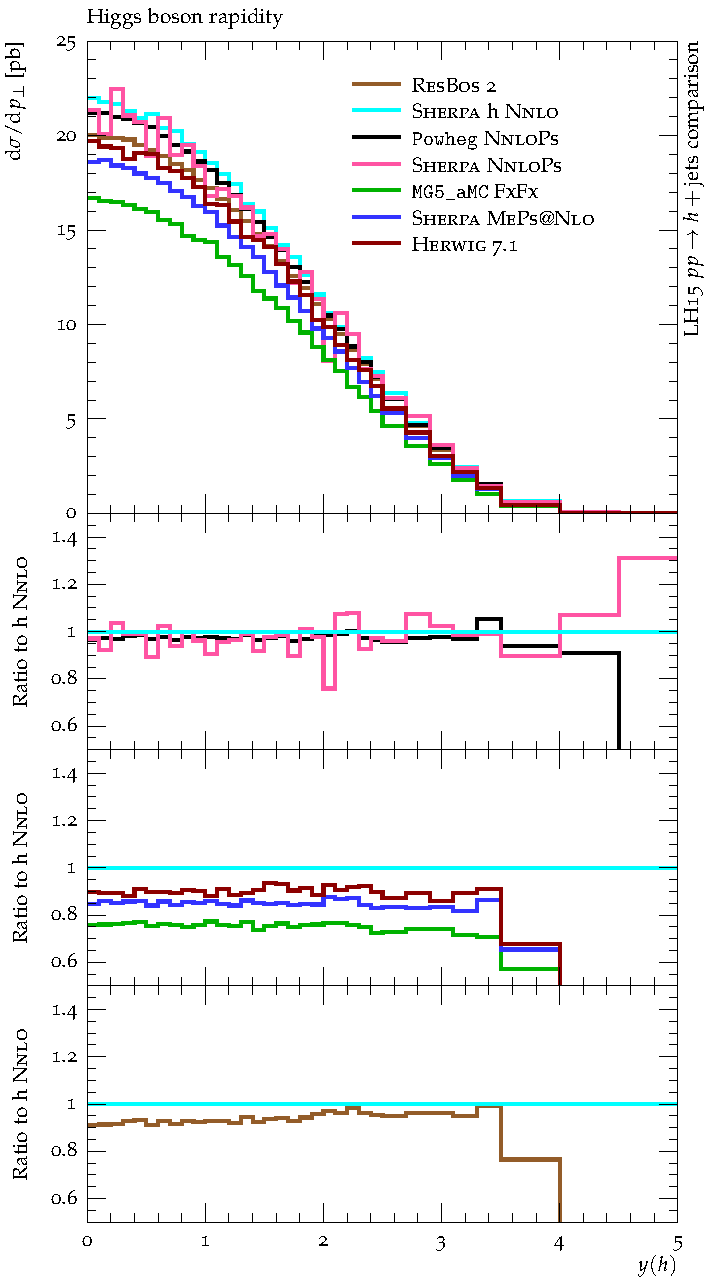
\includegraphics[width=0.47\textwidth]{figures/hjetscomp_u_H_y.pdf}
  \hfill
  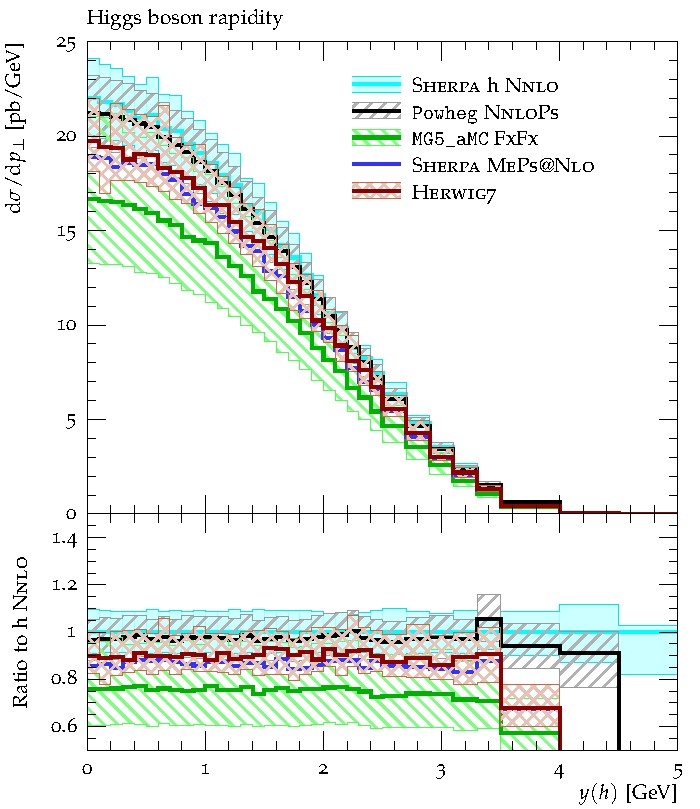
\includegraphics[width=0.47\textwidth]{figures/hjetscomp_H_y.pdf}
  \caption{\label{fig:hjetscomp:results:inclobs:hy}%
    The inclusive Higgs boson rapidity without (left) and with (right)
    uncertainties. To enhance visibility, the \NNLOPS and \MEPSatNLO
    predictions are grouped together and shown with respect to the same reference
    curve in the upper and lower ratio plots, respectively. The
    reference prediction is taken from the NNLO accurate description
    of inclusive $h$ production.}
\end{figure}

We start by examining the inclusive Higgs boson rapidity distribution in
Figure~\ref{fig:hjetscomp:results:inclobs:hy}. While the absolute
predictions are given in the top panel, the plots in the bottom panel
depict the respective ratios to the NNLO prediction. For better
visibility, we have divided the predictions into two groups based on
their simulation type and/or claimed accuracy. The upper ratio plot
contains the NNLO predictions while the lower one shows those obtained
from different strategies to merge matrix elements plus parton showers
at NLO. Overall, we find very good agreement in the description of the
shape of the Higgs boson rapidity distribution. The main source of deviations stems
from the different normalizations given at NNLO or NLO and the
different (core) scale choices. As expected, the \Sherpa \NNLOPS and
\Powheg \NNLOPS results agree well with the fixed order NNLO prediction. 
\Sherpa \NNLOPS' larger fluctuation wrt.\ to \Powheg \NNLOPS' stem from 
it being computed directly rather then reweighted from a NLO computation. 
Consequently, \MGaMC, \Sherpa \MEPSatNLO and \Herwig have slightly lower (NLO)
normalizations.  Here, the \MGaMC scale choice reducing to
$m_h$, rather than $\tfrac{1}{2}m_h$, is clearly noticeable. The upper edge of
the \MGaMC uncertainty band (equal to a scale that reduces to $\tfrac{1}{2}m_h$)
agrees with the central value of the other NLO ME+PS
predictions. There are no major differences in the size of the
uncertainty envelopes, although to some extent, the NNLO scale
uncertainty bands are smaller than those at NLO, as expected. Note
that the NLO-based predictions fall off more rapidly at higher $y$
than the NNLO-based predictions do. This is expected because of the
influence of additional $\ln(1-x)$ corrections present in the
determination of NNLO PDFs. Similar effects can be observed in going
from LO to NLO.

\begin{figure}[t!]
  \centering
  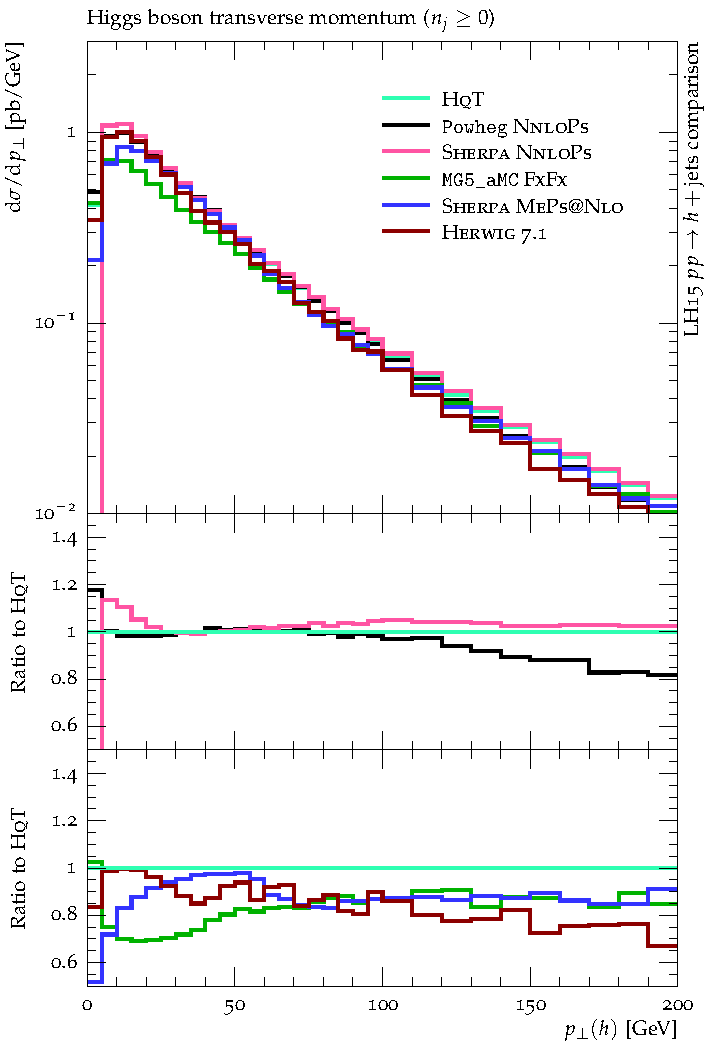
\includegraphics[width=0.47\textwidth]{figures/hjetscomp_u_H_pT_incl.pdf}
  \hfill
  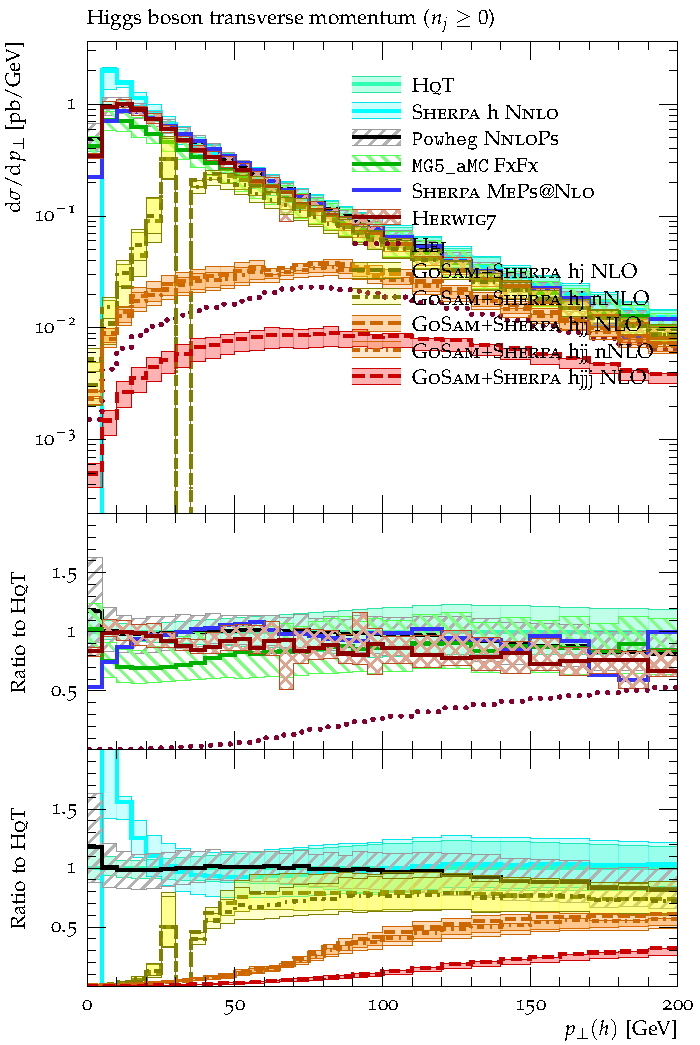
\includegraphics[width=0.47\textwidth]{figures/hjetscomp_H_pT_incl.pdf}
  \caption{\label{fig:hjetscomp:results:inclobs:hpt}%
    The Higgs boson transverse momentum in the inclusive event
    selection without (left) and with (right) uncertainties. For the
    ratios in the bottom panel, the same grouping strategy has been
    used as in Figure~\ref{fig:hjetscomp:results:inclobs:hy}, while
    the reference prediction has been changed from that of pure NNLO
    to the one as given by \HqT.}
\end{figure}

\begin{figure}[t!]
  \centering
  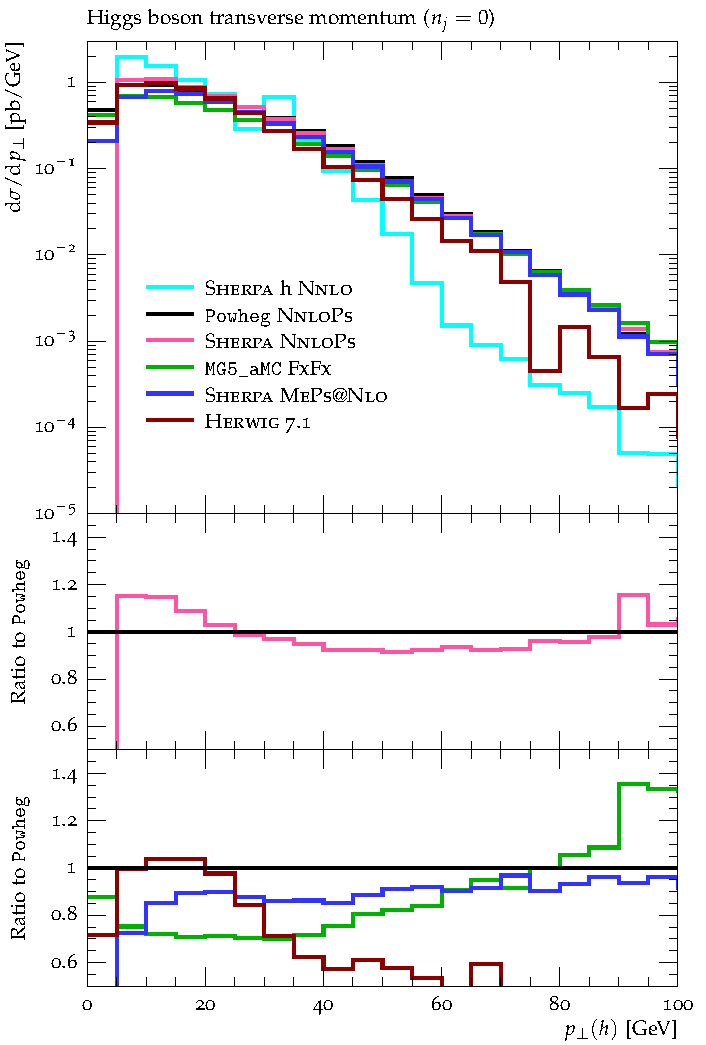
\includegraphics[width=0.47\textwidth]{figures/hjetscomp_u_H_pT_excl.pdf}
  \hfill
  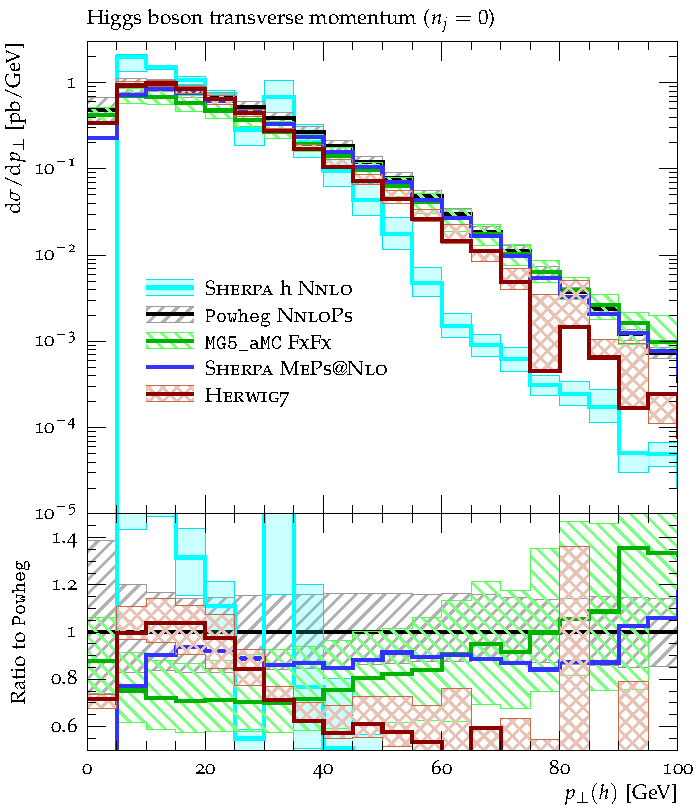
\includegraphics[width=0.47\textwidth]{figures/hjetscomp_H_pT_excl.pdf}
  \caption{\label{fig:hjetscomp:results:exclobs:hpt}%
    The Higgs boson transverse momentum in the exclusive event
    selection (i.e.~in the absence of any jet) without (left) and with
    (right) uncertainties. The bottom panel has been arranged as in
    the previous figure, apart from switching to a new reference curve
    which has been obtained from \Powheg \NNLOPS.}
\end{figure}

In Figures~\ref{fig:hjetscomp:results:inclobs:hpt} and
\ref{fig:hjetscomp:results:exclobs:hpt}, the inclusive and exclusive
(i.e.~vetoing jets above $30$\gev) Higgs boson transverse momentum
distributions are shown, respectively.  For the former, the ratios in
the bottom panel are taken with respect to the \HqT result, while
\Powheg \NNLOPS serves as the reference for the latter case. In
general, good agreement is found, with differences being somewhat more
pronounced in the exclusive case. For the inclusive version of the
$p_\perp(h)$ observable, the good agreement is observed with \HqT,
with some larger deviations evident at very low $p_\perp$. Here the 
resummation properties of the different parton showers dominate the 
spectra of the matched and merged predictions. While the
\Sherpa \NNLOPS curve starts about 15\% higher than both \HqT and \Powheg 
\NNLOPS at low $p_\perp$ it approaches the \HqT results at high $p_\perp$ 
in the fixed-order region. At the same time, \Powheg \NNLOPS follows 
\HqT closely up to scales of $\sim m_h$. Beyond that value, the 
dynamical scale employed \Powheg \NNLOPS accounts for the ensuing 
difference. The multi-jet merged calculations, due to their similar 
scale choices, follow the pattern of the \Powheg \NNLOPS prediction.
Note that the differences in \MGaMC's central scale
choice becomes less significant as the Higgs boson transverse momentum
increases. \Herwig clearly provides the softest spectrum and \Sherpa
as well as \MGaMC predict a noticeably different shape for the Sudakov
suppression at low $p_\perp$. This is not covered by the \HqT
uncertainty envelope. We refrain from showing any fixed order
prediction here because they are neither stable nor reliable at low
$p_\perp$ in the Sudakov region where resummation effects play a 
dominant role.

As shown in Figure~\ref{fig:hjetscomp:results:exclobs:hpt}, the
exclusive version of $p_\perp(h)$ exhibits deviations among the
predictions that become more sizable. The $p_\perp(h)$ distribution 
declines much faster, easily spanning three orders of magnitude 
between zero and $100$\gev. This observable is less straight forward 
than the inclusive $p_\perp$-spectrum as not only Sudakov effects 
dominate the low-$p_\perp$ region, but resummation effects are also 
entering through the veto on any jet activity. It thus necessitates 
both a proper description of small $p_\perp(h)$ region as well as 
jet production. Thus,
this is a stringent test of all predictions combining matrix elements and parton showers (ME+PS), as
the high transverse momentum of the Higgs boson is produced by a
combination of soft jets (those that are below the $30$\gev threshold)
and soft gluon radiation. Note that the comparison is now taken with respect to
\Powheg \NNLOPS. The inclusive 
NNLO calculation is shown to exemplify the failure of a fixed-order 
calculation on both accounts, and, thus, only the parton showered 
predictions are included in the study of the respective differences. 
Among them, apart from the differences already seen in the inclusive 
spectrum, both \NNLOPS calculations agree very well with one another, 
remaining within the 20\% uncertainty bands throughout the spectrum. 
While \Sherpa \MEPSatNLO remains mostly flat with respect to the \NNLOPS 
predictions, both \MGaMC and \Herwig exhibit difference in shape also 
also at larger transverse momenta. In the case
of \Herwig, they even grow larger than 40\%. 
From the resummation (i.e.~parton-shower)
point of view, all predictions are at the same level here, although
formally the \NNLOPS techniques lead to a more accurate description of
the exact zero-jet bin. The NLO merging approaches reduce to an \NLOPS
treatment in this zero-jet bin. It is however hard to infer this
formal difference from the behavior of the scale variation bands as
they are very comparable in size among all predictions. We conclude
that the deviation of the predictions probably provides us with a
better reflection of the true uncertainty.

\begin{figure}[t!]
  \centering
  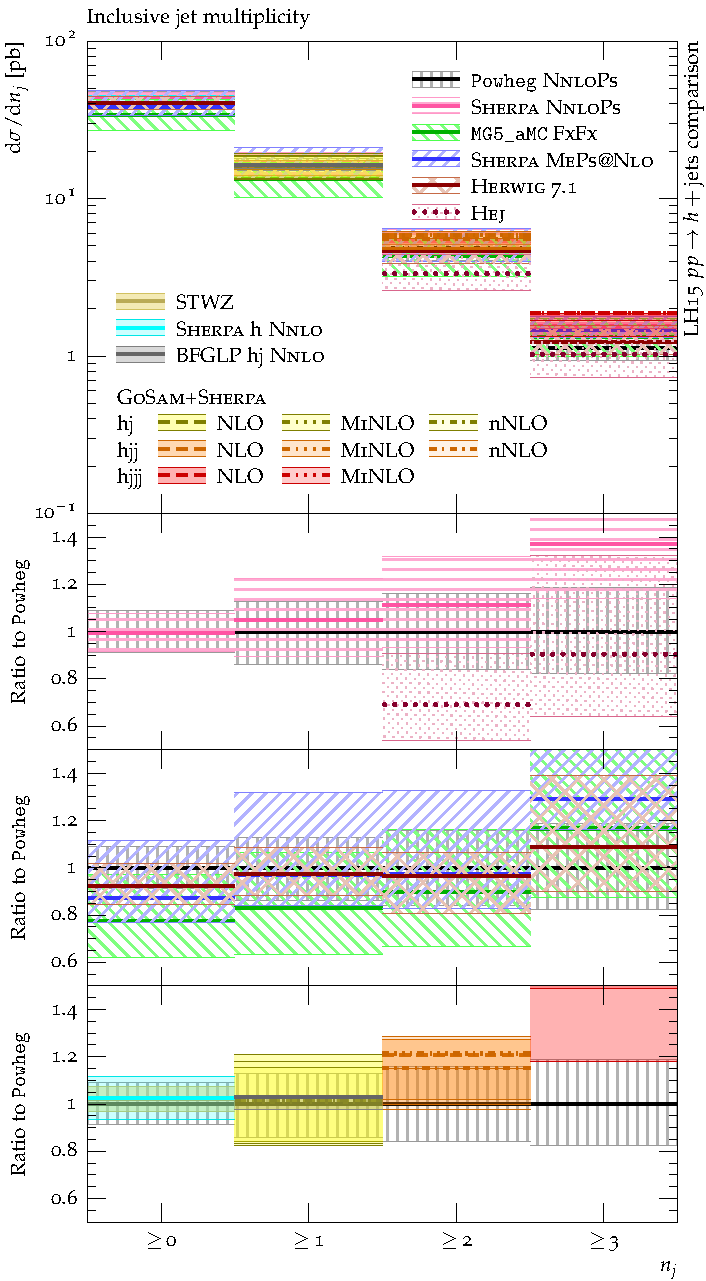
\includegraphics[width=0.47\textwidth]{figures/hjetscomp_NJet_incl_30.pdf}
  \hfill
  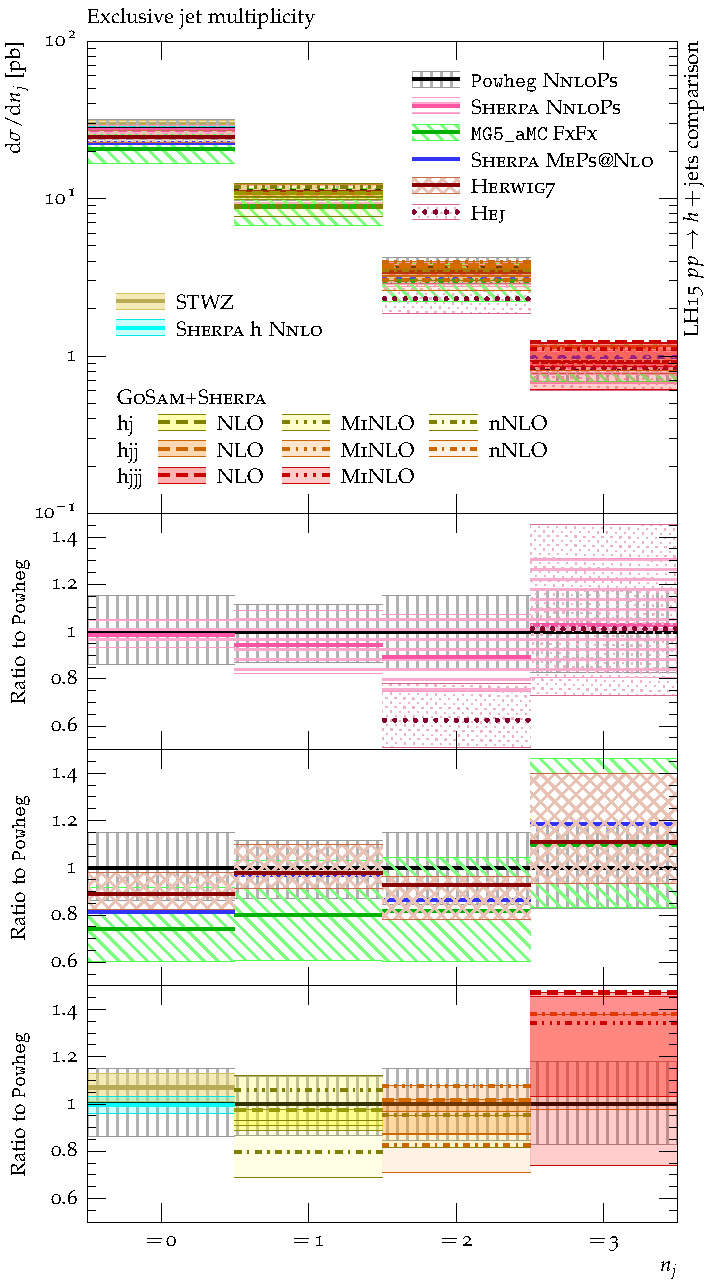
\includegraphics[width=0.47\textwidth]{figures/hjetscomp_NJet_excl_30.pdf}
  \caption{\label{fig:hjetscomp:results:inclobs:njets}%
    The inclusive (left) and exclusive (right) jet multiplicities
    including theoretical uncertainties as predicted by fixed-order
    calculations, resummed calculations, NNLO and NLO Monte Carlos. The
    bottom panel is divided up into three subplots all showing the
    ratios with respect to the \Powheg \NNLOPS prediction. The upper of these plots
    contains the \Hej and \Sherpa \NNLOPS ratios, while the middle one
    includes all NLO merged predictions (\MGaMC, \Herwig and \Sherpa)
    and the lower one shows all those listed in the bottom left legend
    of the main panel.}
\end{figure}

To obtain a first impression of how the different predictions 
compare beyond the zero-jet bins ($n_j\ge0$ and $n_j=0$) we 
look at the various inclusive and exclusive $n_j$ cross sections.
Accordingly, Figure~\ref{fig:hjetscomp:results:inclobs:njets} shows,
to the left, the inclusive ($n_j\ge N$) and, to the right, the
exclusive ($n_j=N$) jet multiplicity distributions up to $N=3$ 
using the previously defined \antikt jets with $p_\perp>30\gev$. Two
statements can be made before discussing the individual results in
more detail: first of all, the agreement between all results is
remarkable, and second, the details of the comparison are barely
altered when going from the inclusive description to the exclusive
description of the jet cross sections, apart from the obvious fact
that the exclusive jet bins always lie below the respective inclusive
jet bins. Although not shown here, when increasing the minimum jet-$p_\perp$ 
threshold to $50\gev$ the picture does not change significantly. 
Again, the bottom panels are split up into several ratio
plots with the common reference provided by the \Powheg \NNLOPS
results. The upper ratio plot depicts the \NNLOPS methods together
with \Hej, which only starts at $N=2$. Due to the scale choices in either 
\NNLOPS calculation they share a common inclusive cross section, with 
\Sherpa rising above \Powheg for higher jet multiplicities. Conversely,
\Hej undershoots by 30\% in the two-jet bin, where all predictions in this 
panel are LO accurate. In the three-jet bin, \Hej retains the LO accuracy 
while in both \NNLOPS calculations it is described by their respective 
parton showers only. Naturally, here the differences between the \NNLOPS 
predictions are largest. Please note, that the respective parton showering 
uncertainties are partially incorporated in the \Sherpa \NNLOPS uncertainty 
estimate while they are not assessed for \Powheg, resulting in a very flat 
uncertainty band. The central ratio plot confronts the NLO
matched and merged predictions with each other and against the common reference 
\Powheg \NNLOPS. All these predictions have claim NLO accuracy for $N=0,1,2$ 
and overlap well within uncertainties where the lower value for \MGaMC can 
again be attributed to the different scale choice. For $N=3$ only the \Sherpa 
\MEPSatNLO prediction retains its NLO accuracy while \MGaMC and \Herwig 
revert to LO, which is nicely reflected in the uncertainty estimates. 
Unsurprisingly, in the $N=3$ case, described by the reference with its 
parton shower only, all three NLO merged calculations predict larger 
cross sections.

Lastly, fixed-order predictions are shown for all jet multiplicities
at NLO (provided by \GoSam+\Sherpa) for the $1$-jet, $2$-jet and
$3$-jet bins and at approximate NNLO (labeled nNLO, provided by \Loopsim) 
for the $1$-jet and $2$-jet bins.
Complete NNLO predictions are shown for the 0-jet inclusive and
exclusive bins using \Sherpa without PS and for the 1-jet inclusive
bin using the prediction of Boughezal et al.~(BFGLP).
In addition, the zero-jet bin comparison
also contains the resummation prediction of Stewart et
al.~(STWZ) whereas the comparison for non-zero jet bins also
shows the \Minlo enhanced NLO calculations. All of the above are
grouped together in the lower ratio plot. For the zeroth bin, nice
agreement can be found between \Powheg and \Sherpa \NNLOPS as well as
the STWZ approach; the uncertainties also are of comparable
size. In the $1$-jet case, \Powheg (being NLO accurate in this bin)
resides 10\% above the pure NLO prediction, which simply is triggered
by the different scale choices. Unlike the inclusive Higgs boson
production case, the NNLO corrections for inclusive $1$-jet production
are small -- slightly negative for the central scale choice as given
in Eq.~(\ref{eq:bfglpScale}). There is a notable decrease in the scale
uncertainty with respect to the NLO band given by \GoSam+\Sherpa. The $2$-jet bin
shows the \GoSam NLO prediction just slightly above \Powheg, which
gives a LO prediction in this case. For the same reason, the \Powheg
uncertainties in the higher jet multiplicities are probably
underestimated. In the $3$-jet bin (both inclusive and exclusive), the
\GoSam+\Sherpa and \Sherpa \MEPSatNLO predictions clearly signal the absence of 
NLO corrections 
in the other predictions. The \Loopsim results for $h+j$ and
$h+jj$ are always somewhat below the respective \GoSam result
though the relatively large MC generation cut of $25$ \gev mean
the total rates predicted using \Loopsim should be interpreted with care.
Furthermore, compared to the NLO benchmark, the \Minlo approach
predicts 10-20\% larger cross sections for all non-zero jet bins.
Note that the \Minlo ratio for inclusive
$h+jjj$ turns out to be outside the plot range appearing at around
$1.65$ where the lower edge of the uncertainty band is seen kicking in
at a ratio value of $1.5$. In the cases where NNLO precision is available
the reduction in scale uncertainty is clear. For $n_j\geq1$ the variation around
$\mu_R=\sqrt{\Sigma_T}/2$ is about $5.5\%$ while for $n_j\geq0$ it is about $10\%$
around $\mu_R=m_h/2$. The latter result can be improved using the N${}^3$LO prediction
of Anastasiou et al. \cite{Anastasiou:2015ema} to only a few percent. In order to compare more
easily with results presented previously in the literature we give numerical values at NLO and NNLO
for different scale choices in Table \ref{tab:H1jXS}. As observed previously \cite{Boughezal:2015dra},
the convergence of the total cross-section is improved for scales that limit to $m_h/2$. The dynamical scale
of $\sqrt{\Sigma_T}$ defined in eq. \eqref{eq:bfglpScale} is slightly harder than the fixed scale given the
minimum jet $p_{T,j}>30$. On the other hand it is softer than $\hat{H}_T'$ defined in eq. \eqref{eq:hthatprime} which explains
the differences at NLO.

\begin{table}
  \centering
  \begin{tabular}{c||c|c|c}
    order \vphantom{$\int\limits_a^b$} & $\mu_R=\mu_F=\tfrac{1}{2}\,m_h$ & $\mu_R=\mu_F=\tfrac{1}{2}\,\hat{H}_T'$ & $\mu_R=\mu_F=\tfrac{1}{2}\,\sqrt{\vphantom{\big[}\Sigma_T}$ \\
    \hline\hline
    NLO \vphantom{$\int\limits_a^b$}  & $17.0^{+3.0}_{-2.9}$ pb & $13.5^{+2.0}_{-2.1}$ pb & $16.2^{+3.1}_{-2.8}$ pb \\\hline
    NNLO \vphantom{$\int\limits_a^b$} & -     & -     & $16.4^{+0.0}_{-0.9}$ pb \\
    \hline
  \end{tabular}
  \caption{
    The total cross-section for inclusive production of a Higgs boson and 
    one additional jet using different core scale choices.  The two 
    dynamical scales are $\hat{H}_T'=m_{T,h} + \sum_{\rm partons} p_T$ 
    (see also eq.~\eqref{eq:hthatprime}) and 
    $\Sigma_T = m_h^2 + \sum_{\rm jets} p_T^2$ 
    (see also eq.~\eqref{eq:bfglpScale}).
  }
  \label{tab:H1jXS}
\end{table}


\subsection{One-jet observables}
\label{sec:hjetscomp:results:1jobs}

In this section, we move away from the fully inclusive picture and
require the presence of at least one jet associated with the Higgs
boson. In some cases we also ask for the predictions where exactly one
jet is being resolved. Recall that the jets are defined based on the
anti-$k_T$ algorithm using $R=0.4$; they furthermore have to obey the
criteria that $p_\perp(j)>30\gev$ and $|\eta(j)|<4.4$. The set of
observables presented here includes the transverse momentum
distributions of the Higgs boson $h$, the leading jet $j_1$ and the
$hj_1$ two-body system as well as the rapidity spectrum of the leading
jet.

\begin{figure}[t!]
  \centering
  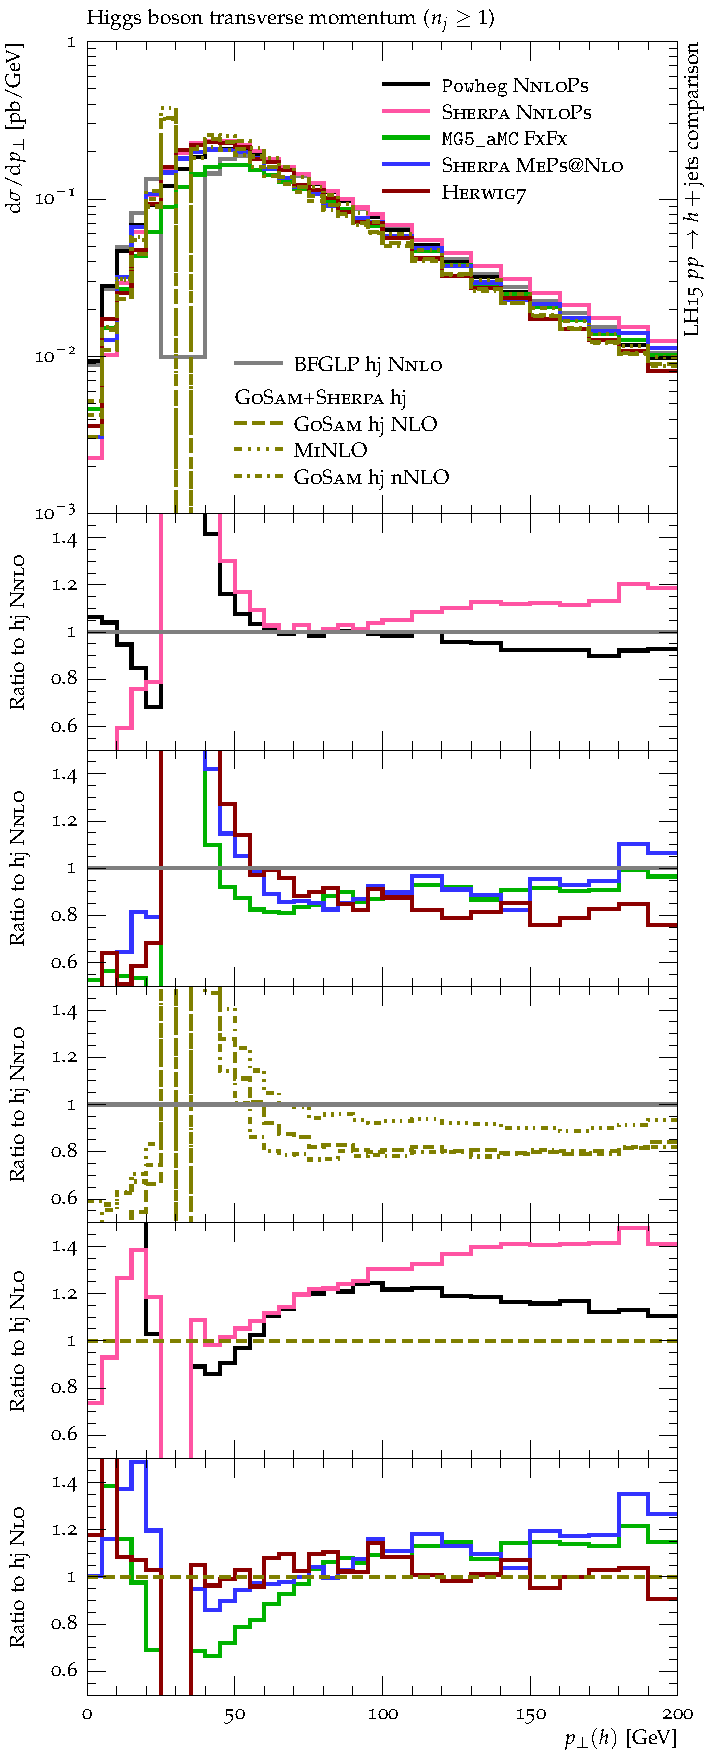
\includegraphics[width=0.47\textwidth]{figures/hjetscomp_u_H_j_pT_incl.pdf}
  \hfill
  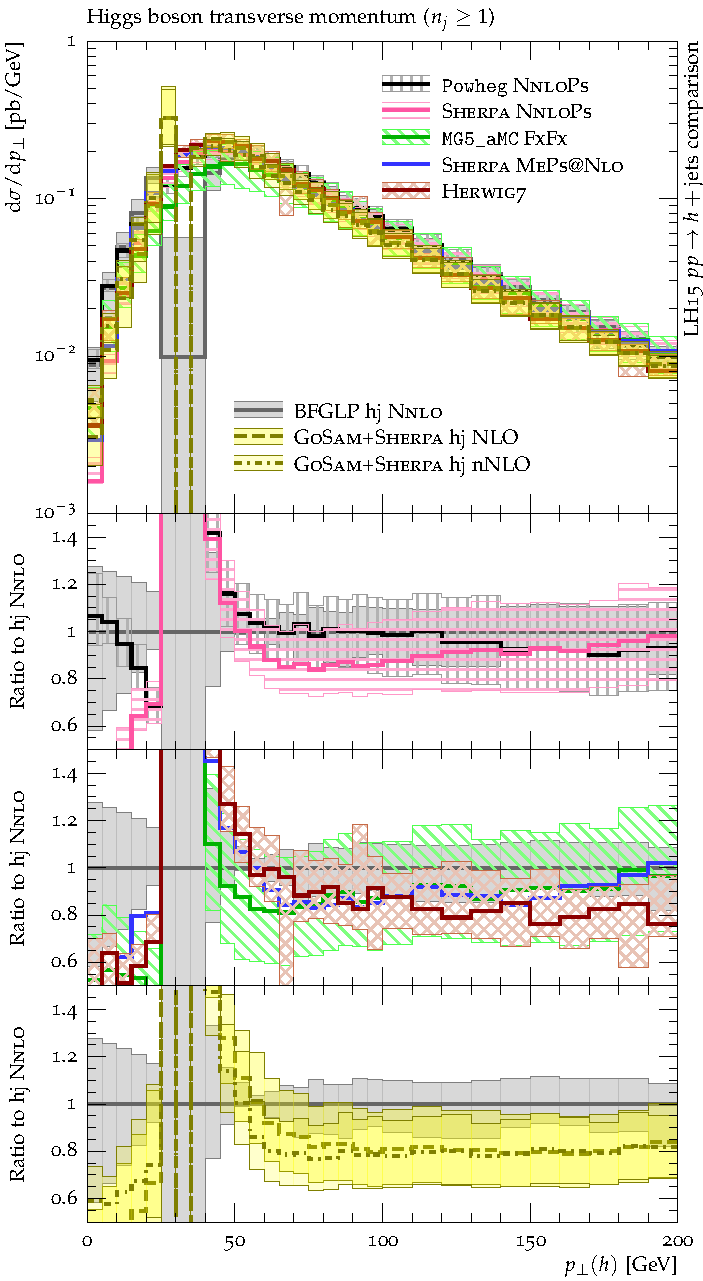
\includegraphics[width=0.47\textwidth]{figures/hjetscomp_H_j_pT_incl.pdf}
  \caption{\label{fig:hjetscomp:results:1obs:hpt}%
    The Higgs boson transverse momentum in the presence of at least
    one jet without (left) and with (right) uncertainty bands. The
    ratio plot panel is divided into five parts where the upper three
    exhibit the ratios wrt.~the \Powheg \NNLOPS result while the lower
    two show them wrt.~the NLO calculation for $h\pl1$~jet as
    provided by \GoSam+\Sherpa. The grouping in the ratio plots has
    been arranged to separately compare with each other the \NNLOPS
    predictions (first and fourth subplot), the NLO merging
    predictions (second and fifth subplot) and the fixed-order
    predictions (subplot in the middle).}
\end{figure}

\begin{figure}[t!]
  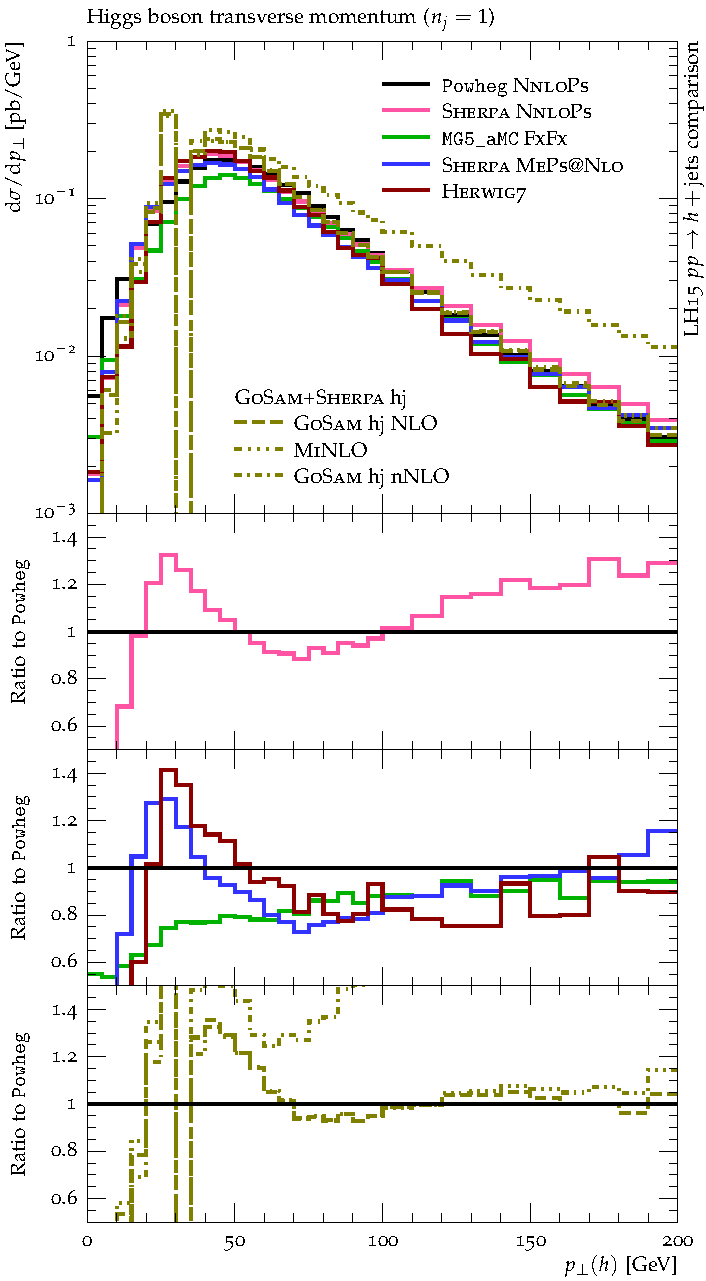
\includegraphics[width=0.47\textwidth]{figures/hjetscomp_u_H_j_pT_excl.pdf}
  \hfill
  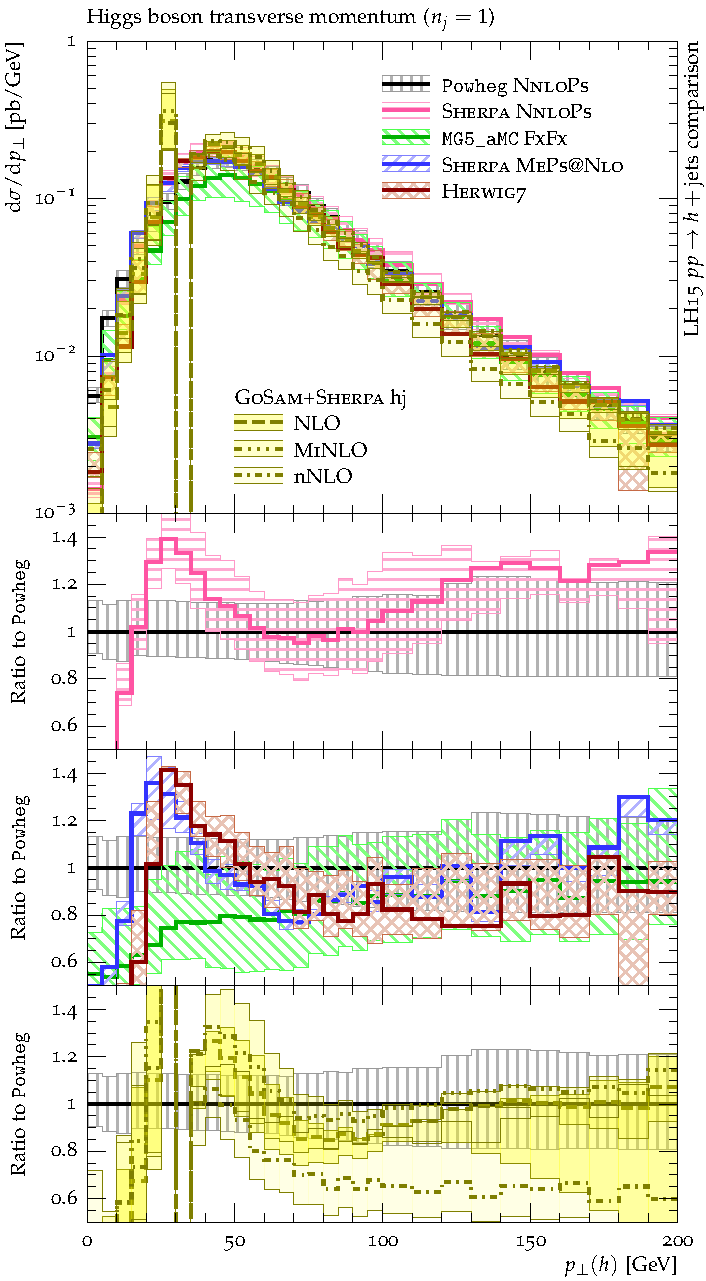
\includegraphics[width=0.47\textwidth]{figures/hjetscomp_H_j_pT_excl.pdf}
  \caption{\label{fig:hjetscomp:results:1obs:hpt_excl}%
    The Higgs boson transverse momentum in the presence of exactly one
    jet without (left) and with (right) uncertainty bands. The ratio
    plot panel is divided into three parts all of which depicting the
    corresponding ratios wrt.~the \Powheg \NNLOPS result. From top to
    bottom, the predictions are grouped such that the \NNLOPS results,
    the ME+PS results at NLO and the fixed-order results are compared
    directly in the first, second and third ratio plot, respectively.}
\end{figure}

The Higgs boson transverse momentum distribution in the presence of at
least one jet is shown in
Figure~\ref{fig:hjetscomp:results:1obs:hpt}. The exclusive version of
this plot, i.e.~where one requires the $hj$ final states to be exact,
is presented in Figure~\ref{fig:hjetscomp:results:1obs:hpt_excl}.  As
for the zero-jet cases discussed earlier in
Figures~\ref{fig:hjetscomp:results:inclobs:hpt}~and~\ref{fig:hjetscomp:results:exclobs:hpt},
the one-jet $p_\perp(h)$ variables are prone to large, maybe sligthly
stronger, Sudakov effects that arise at low $p_\perp$ but also beyond
this area, in particular for the exclusive final states. Moreover, the
Sudakov shoulder effect can be observed for all fixed-order
predictions shown here. The jet-$p_\perp$ threshold leads to a
non-smooth behaviour of the $p_\perp(h)$ observable at LO, and
therefore to the existence of a critical point at $30\gev$ for which
the cancellations between real and virtual soft-gluon singularities
will be imperfect at any given fixed, higher order in perturbation
theory~\cite{Catani-Webber}. For the NNLO $hj$~\cite{.} prediction, an
averaging procedure has been used to dampen the effect around the jet
threshold while for the NLO predictions, the large oscillations are a
clear indication of the instability emerging at the jet threshold.
Comparing the different fixed-order predictions, which is done best by
looking at the ratio plot in the middle, noticeable differences only
occur between the NNLO prediction and the four NLO predictions as
obtained from \Powheg and the three version of \GoSam+\Sherpa (pure
NLO, \Minlo and \Loopsim). The NNLO tail is harder by about 15\% which
is expected since the $p_\perp$ tail is affected by multi-jet
contributions. The NNLO treatment includes these contributions to a
larger extent, as it respectively includes $h\pl2$-jet and
$h\pl3$-jet contributions at the NLO and LO. Another difference is
that for $p_\perp(h)\to0$, the NNLO description gets closer to the
resummed result (\Powheg) because it reproduces more terms of the
all-orders expression than the pure NLO predictions do. However, it
can be noticed that apart from \Powheg and BFGLP's NNLO $hj$
calculation, all other approaches predict a more steeply falling
shoulder when $p_\perp(h)\to0$ resulting in a significantly lower
intercept point with the $\hat y$-axis.

\Todo{Don't have a good explanation why Powheg and BFGLP are so
  different regarding intercept ... anybody else?}

For larger $p_\perp(h)$ values, $p_\perp(h)>70\gev$, in general there
is good agreement between \Powheg, \MGaMC, \Sherpa and the NLO curves;
this can be expected as these predictions are all NLO-accurate. As
before, \Herwig tends to be softer, whereas \MGaMC using the nominal
$\tfrac{1}{2}m_h$ core scale turns out to be harder by almost 40\% as
inidcated by the upper edge of the corresponding uncertainty band, see
second or last subplot to the right in
Figure~\ref{fig:hjetscomp:results:1obs:hpt}. \Sherpa's \NNLOPS
prediction also features a harder tail than \Powheg owing to the
different scale setting procedures employed by the two approaches.
While in \Powheg the scale setting is accomplished through the \Minlo
procedure, \Sherpa uses the fixed scale choice of $\tfrac{1}{2}m_h$
and therefore enhances the $p_\perp$ tail wrt.~\Powheg's result. We
furthermore observe that apart from the BFGLP NNLO computation, all
uncertainty envelopes are of similar size, which does not come as a
surprise because all of these predictions are effectively given at
NLO. The NNLO uncertainty band (shown in grey) is found to be
significantly smaller. Comparing the second and last ratio plots with
each other, we also notice that the ME+PS predictions are in better
overall agreement with the pure NLO prediction given by \GoSam+\Sherpa
than they are in agreement with \Powheg. This may be a result of the
global scale choice, cf.~Eq.~(\ref{eq:bfglpScale}), used by the NLO
calculation as it seems to be a more decent proxy to the ME+PS local
and dynamical scale setting procedures than it is one to the \Powheg
approach.

For the exclusive one-jet case, we reduce the number of ratio plots
and show only those that display the ratios to \Powheg in the same way
as before. Note that for the exclsuive version of the observable, the
NNLO result is not available turning this comparison into one between
NLO-accurate predictions, except for the NNLO-approximate result given
by \Loopsim, labelled \GoSam $hj$ nNLO.
Figure~\ref{fig:hjetscomp:results:1obs:hpt_excl} clearly shows that
the differences among the results are very similar to those discussed
in the inclusive case; they are however pronounced such that the
deviations wrt.~the \Powheg \NNLOPS prediction for $h$ production
become larger for the full tranverse momentum range. There is one
exception to this: \Loopsim predicts a softer tail of the $p_\perp(h)$
distribution by about 20\%. \Todo{Not quite sure why that is.}

\begin{figure}[p!]
  \centering
  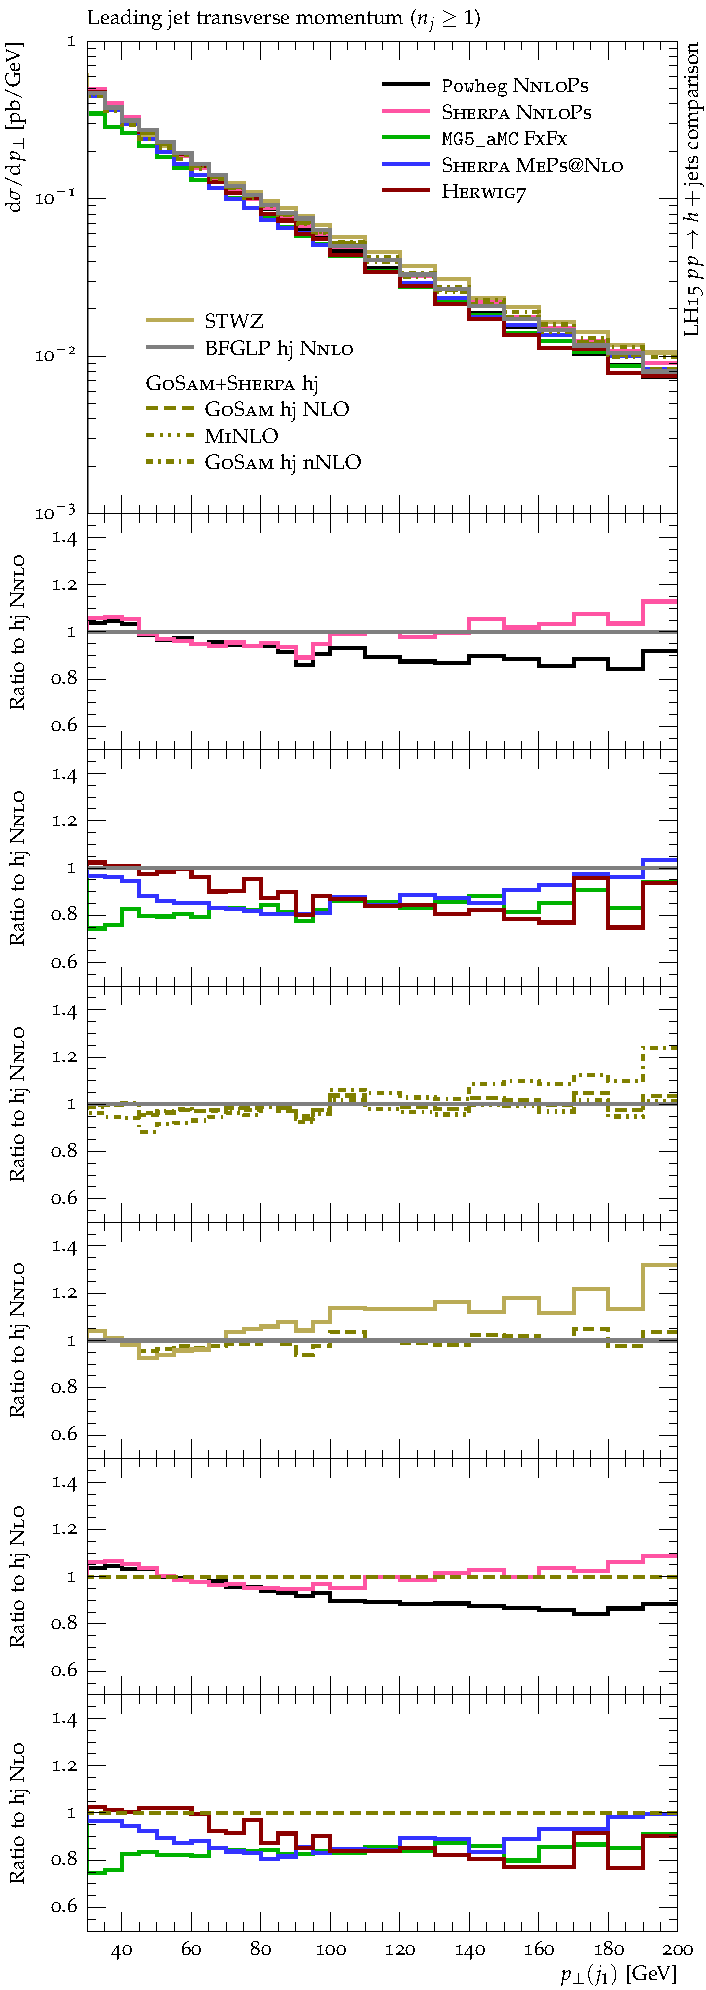
\includegraphics[width=0.47\textwidth]{figures/hjetscomp_u_jet1_pT_incl.pdf}
  \hfill
  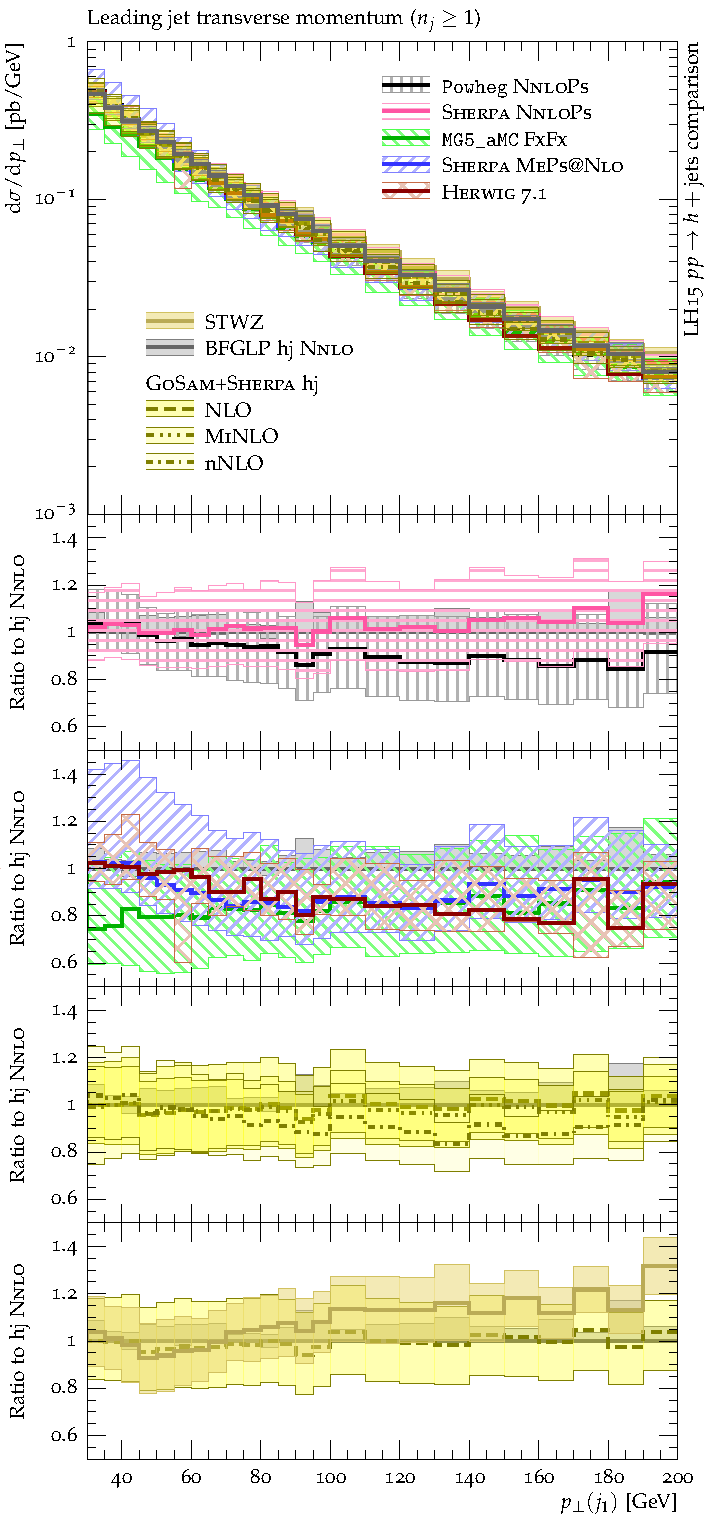
\includegraphics[width=0.47\textwidth]{figures/hjetscomp_jet1_pT_incl.pdf}
  \caption{\label{fig:hjetscomp:results:1obs:j1pt}%
    The leading jet transverse momentum distribution for
    $h\pl\ge1$-jet production, to the right (left) shown with
    (without) the uncertainty bands provided by the various
    calculations. The part below the main plot contains ratio plots
    taken wrt.~the NNLO result of the BFGLP group (subpanel one
    through four) and the NLO result given by \GoSam+\Sherpa (lowest
    two subpanels) following the same strategy for grouping the
    predictions as before (\NNLOPS versus NLO ME+PS versus fixed-order
    results). Note the layout of the first and last two subpanels is
    the same, apart from exchanging the reference.}
\end{figure}

\begin{figure}[t!]
  \centering
  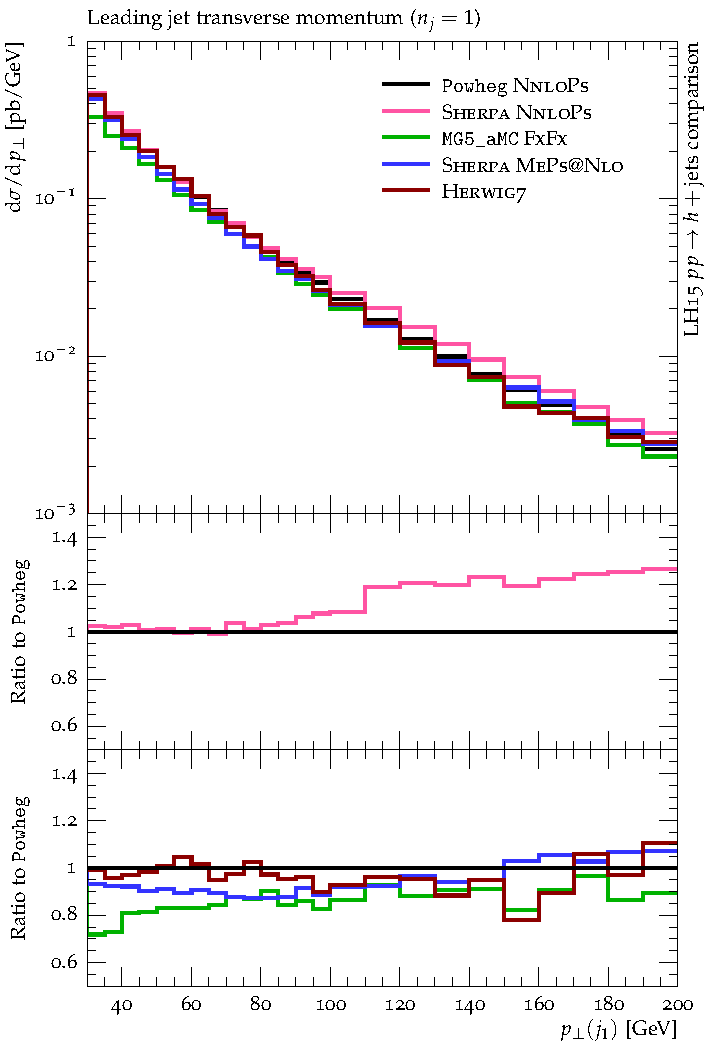
\includegraphics[width=0.47\textwidth]{figures/hjetscomp_u_jet1_pT_excl.pdf}
  \hfill
  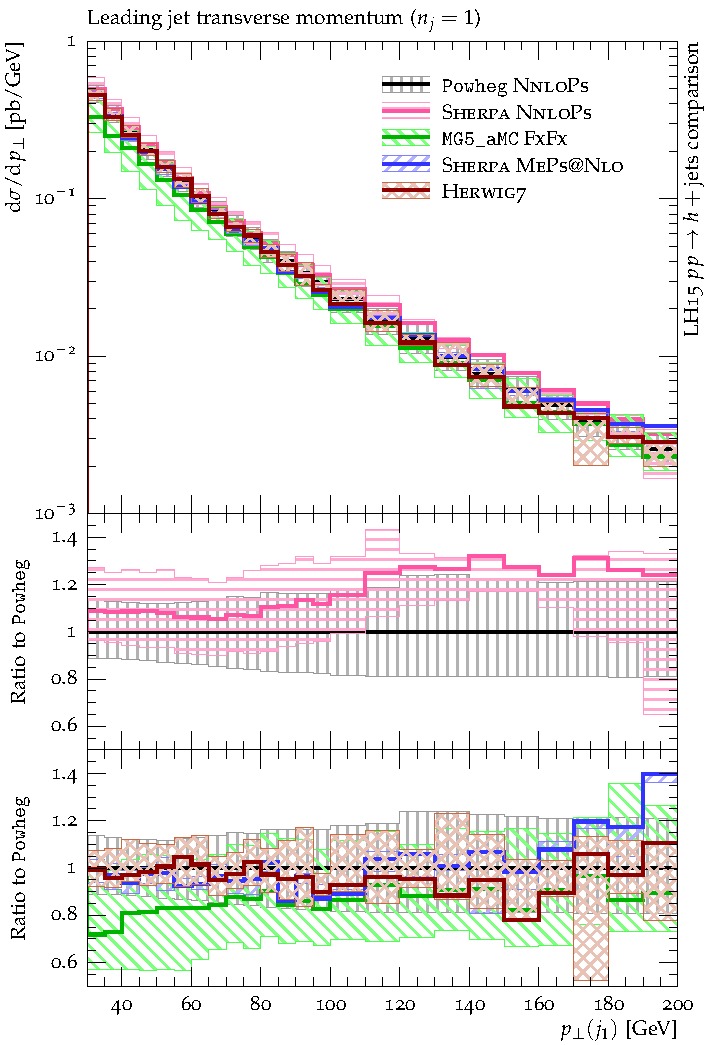
\includegraphics[width=0.47\textwidth]{figures/hjetscomp_jet1_pT_excl.pdf}
  \caption{\label{fig:hjetscomp:results:1obs:j1pt_excl}%
    The leading jet transverse momentum distribution for exclusive
    $h\pl1$-jet production, to the right (left) shown with (without)
    the uncertainty bands provided by the various calculations. Ratio
    plots are displayed in the lower part of the plot using the
    \Powheg \NNLOPS result for $h$ production as their reference.
    Predictions are grouped in similar fashion to the previous plots.}
\end{figure}

Next we discuss the leading jet transverse momentum distribution for
$h\pl\ge1$-jet final states. For this type of observable, we do not
expect large Sudakov effects (i.e. shifts owing to parton
showering/resummation). The impact of jet veto logarithms (owing to
the restriction that all jets be greater than $30\gev$) has been
examined and found to be reasonably small at NLO and
NNLO~\cite{monni}. \Todo{provide numbers from Monni?} \Todo{MS: Dowe have any?}
In the exclusive jet case, the $p_\perp(j_1)$ variable however is
prone to larger resummation effects, and we note that the scale
uncertainties shown will not reflect the true uncertainty. The
inclusive jet results for all approaches are shown in
Figure~\ref{fig:hjetscomp:results:1obs:j1pt} including the NNLO
prediction of the BFGLP group and the prediction of Stewart, Tackmann
et al. Figure~\ref{fig:hjetscomp:results:1obs:j1pt_excl} depicts the
exclusive one-jet case presenting the results obtained by the Monte
Carlo tools only; no fixed-order predictions are shown. Accordingly,
different reference predictions (NNLO and \Powheg) are used in the
ratio plots associated with
Figures~\ref{fig:hjetscomp:results:1obs:j1pt} and
\ref{fig:hjetscomp:results:1obs:j1pt_excl}; for the inclusive one-jet
scenario, two additional ratio plots are displayed using the NLO
\GoSam+\Sherpa reference but otherwise correspond to the upper two
ratio plots. \Todo{these last two rplots may be removed since BFGLP
NNLO == GoSam NLO here} Overall we find a rather remarkable agreement
between all results where the largest deviations rarely exceed the
20\% mark. For the exclusive lead-jet transverse momentum distribution
of Figure~\ref{fig:hjetscomp:results:1obs:j1pt_excl}, this means that
all predictions are in reasonably good agreement with \Powheg. The
\MGaMC prediction is lower than \Powheg for basically the entire
transverse momentum range, again because of the central scale choice
being higher than in the other approaches. For the inclusive lead-jet
transverse momentum spectrum (see
Figure~\ref{fig:hjetscomp:results:1obs:j1pt}), the remarkable
agreement implies that all predictions indeed lie within each other's
uncertainty bands. The quoted uncertainties are similar in size, with
values at and around the 20\% level, and only those of the BFGLP NNLO
calculation and the \MGaMC simulation using the higher central scale
turn out to be significantly smaller and somewhat wider, respectively.

Despite the good agreement seen among all predictions in
Figure~\ref{fig:hjetscomp:results:1obs:j1pt}, it is worthwhile to go
through the ratio plots and discuss some of the interesting features.
In the second panel, the two \NNLOPS predictions are compared to the
NNLO $h\pl\ge1$-jet prediction. The agreement among all three is
good at low transverse momentum, but at higher $p_\perp(j_1)$ there is
a tendency for \Sherpa \NNLOPS to be slightly higher and \Powheg
NNLOPS to be slightly lower, resulting in a 20\% net difference
between the two. Again, this is a result of using
$\mu=\tfrac{1}{2}m_h$ within \Sherpa versus using \Minlo within the
\Powheg approach. In the third panel, \Herwig, \Sherpa and \MGaMC
(taking into account its larger limit scale) agree reasonably well
with each other over the entire transverse momentum range, but fall
about 15\% low wrt.~the BFGLP prediction in the mid-range of the
$p_\perp$ distribution. The fourth panel shows that there is almost no
difference in normalization nor shape between the NNLO and the NLO
$h\pl\ge1$-jet predictions using the given scale choice,
cf.~Eq.~(\ref{eq:bfglpScale}). This extends to the \Minlo reweighted
NLO result and the nNLO prediction provided by \Loopsim, although the
latter is somewhat softer. In the fifth panel, the STWZ prediction
agrees with the NNLO prediction at low $p_\perp$, but rises up to 30\%
higher at the largest $p_\perp$ values. As mentioned earlier, in the
bottom two panels, comparisons are made to the NLO $h\pl\ge1$-jet
prediction, basically reproducing the results of the first and second
subpanel as the similarity of the NNLO and NLO curves is perfect for
the scale choice given by Eq.~(\ref{eq:bfglpScale}).

In summary, the fixed-order NNLO prediction of the BFGLP group, which
has the best theoretical uncertainties available, is in good agreement
with the \Sherpa predictions (\NNLOPS and \MEPSatNLO), and to a
somewhat lesser extent with the other ME+PS predictions. The level of
moderate disagreements observed with the latter may be due to the
somewhat different scale choices that are still important at
NLO. There is no sign of any serious impact of the merging of the
fixed-order predictions with parton showers, as expected for such an
inclusive cross section.

\begin{figure}[t!]
  \centering
  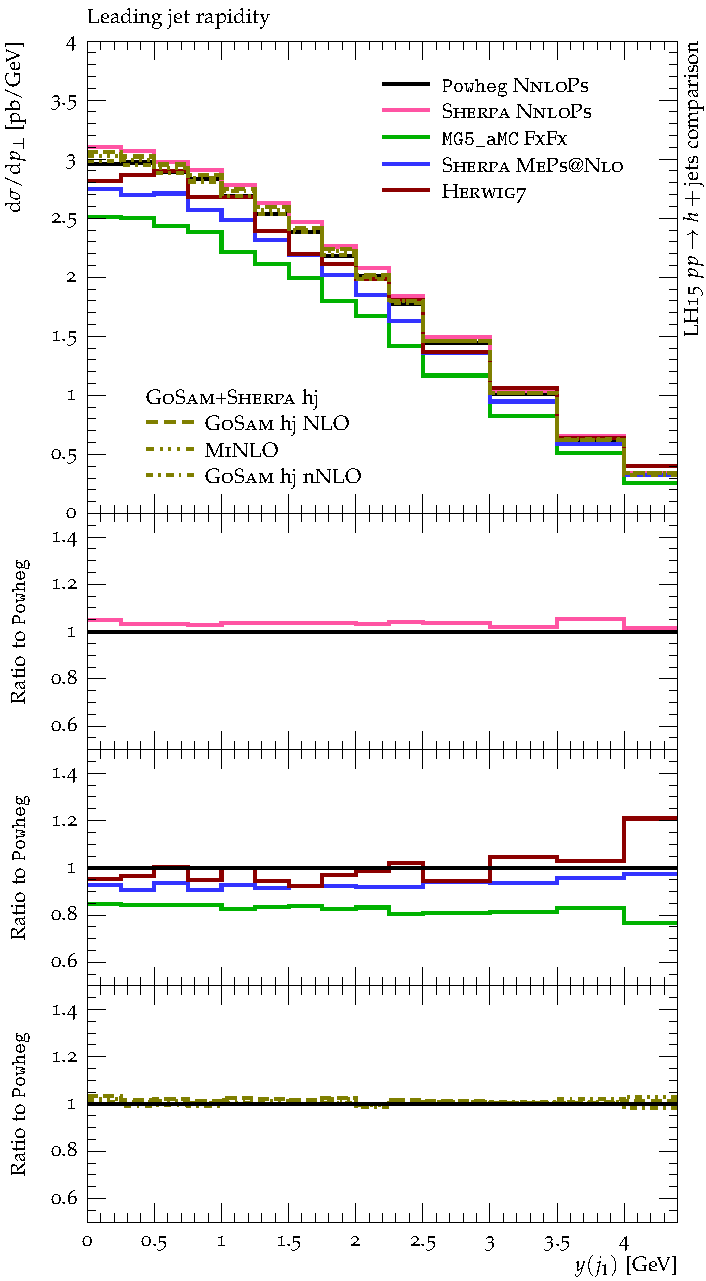
\includegraphics[width=0.47\textwidth]{figures/hjetscomp_u_jet1_y.pdf}
  \hfill
  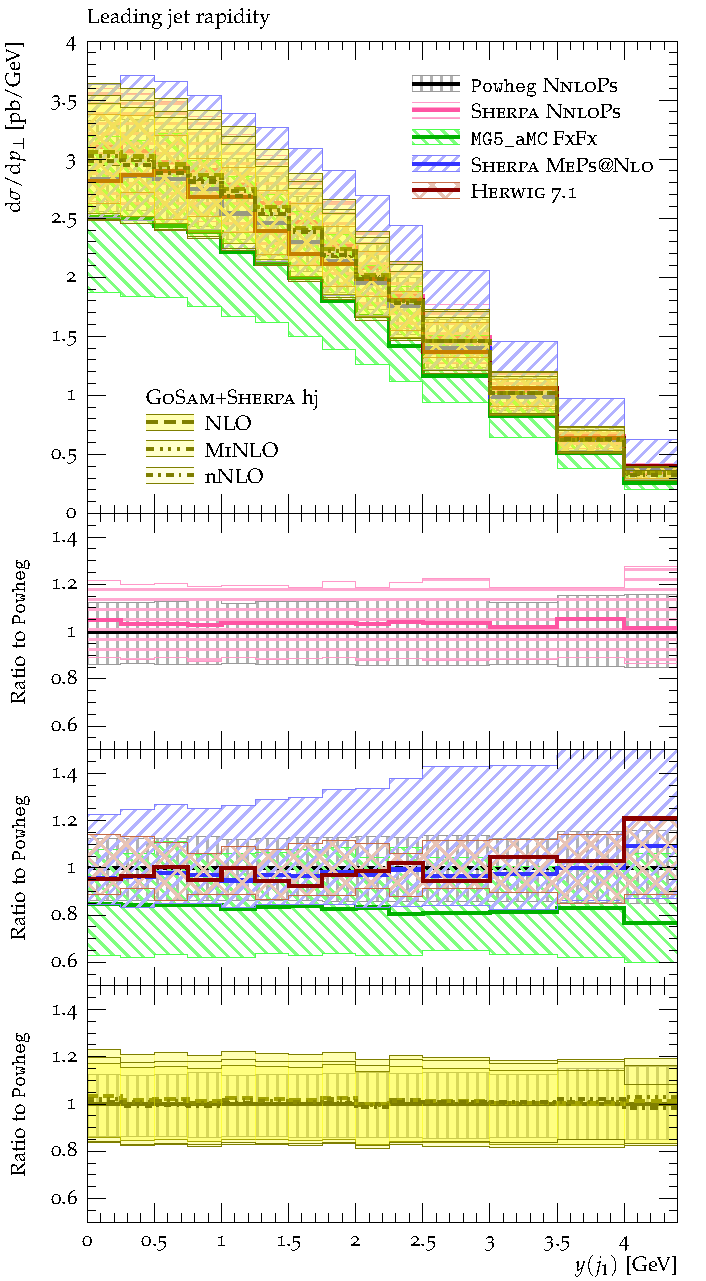
\includegraphics[width=0.47\textwidth]{figures/hjetscomp_jet1_y.pdf}
  \caption{\label{fig:hjetscomp:results:1obs:j1y}%
    The rapidity distribution for the leading jet in $h\pl\ge1$-jet
    production, shown without (left) and with (right) theoretical
    uncertainties. Ratio plots are displayed in the lower part of the
    plot using the \Powheg \NNLOPS result for $h$ production as their
    reference. Predictions are grouped, from top to bottom, according
    to the categories \NNLOPS, ME+PS at NLO and NLO fixed order.}
\end{figure}

Did we talk about great agreement in the previous case where we
discussed the $p_\perp(j_1)$ distribution, the agreement found for the
rapidity distribution of the lead jet, $y(j_1)$, is magnificient, as
demonstrated by Figure~\ref{fig:hjetscomp:results:1obs:j1y}. We were
to expect that due to the $p_\perp(j_1)$ agre and earlier findings
concerning $y(h)$, see Figure~\ref{fig:hjetscomp:results:inclobs:hy}.
We basically do not observe any shape differences, and the rate
differences follow the already established pattern where most
noticeably the \MGaMC cross section is reduced owing to their choice
of using a higher central scale. Again, uncertainty envelopes are
by and large similar in size and do not point to any shape changes
when varying the scales; \Herwig's band is slightly narrower while
\MGaMC's band is somewhat wider compared to all other NLO-accurate
predictions.

\begin{figure}[t!]
  \centering
  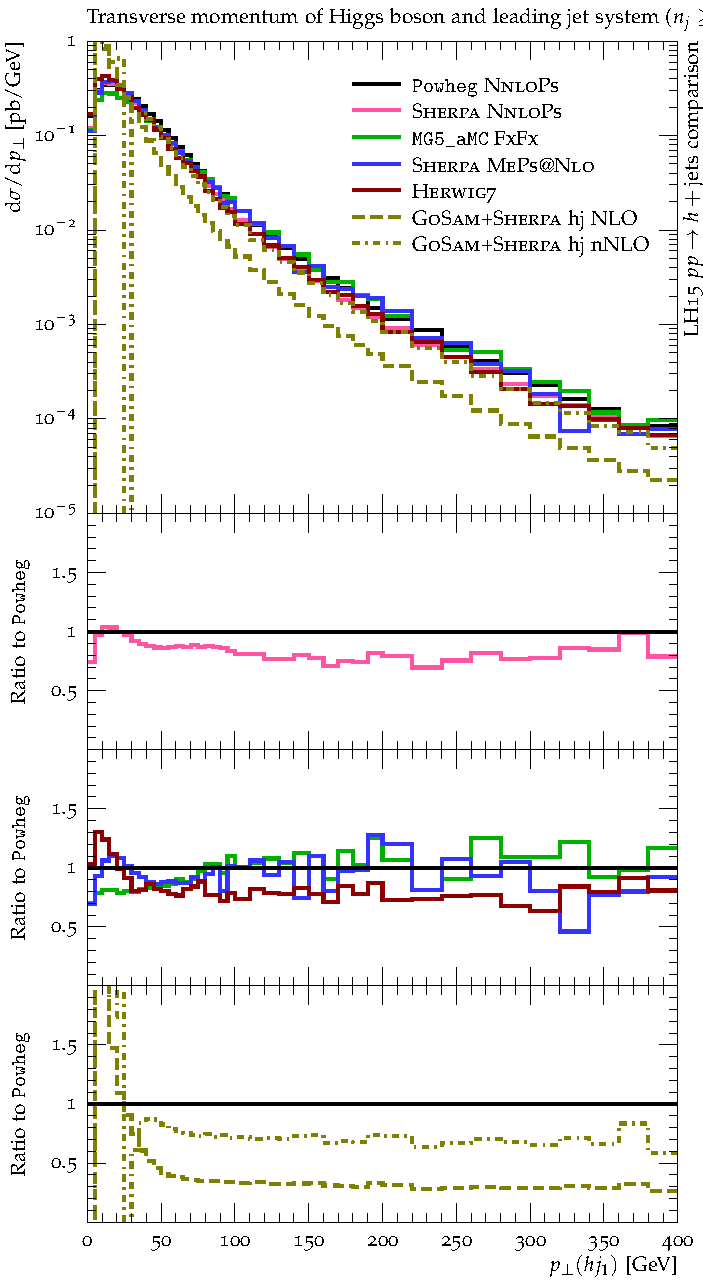
\includegraphics[width=0.47\textwidth]{figures/hjetscomp_u_Hj_pT_incl.pdf}
  \hfill
  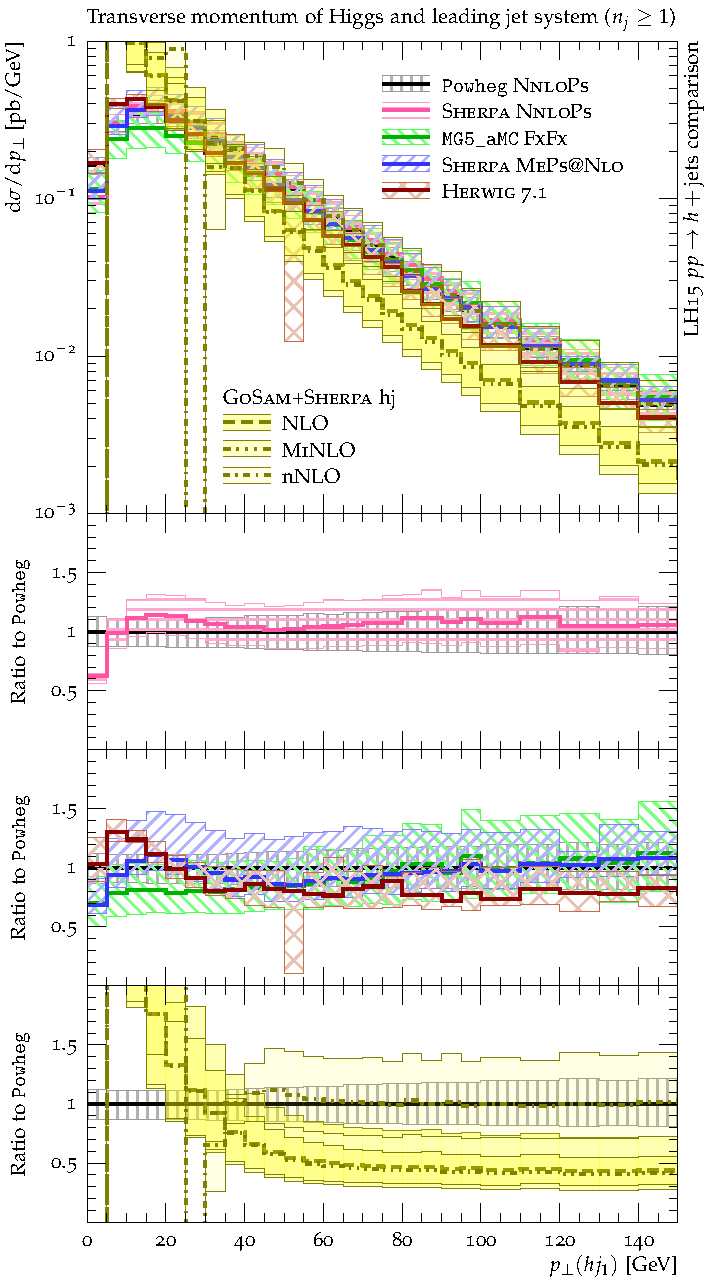
\includegraphics[width=0.47\textwidth]{figures/hjetscomp_Hj_pT_incl.pdf}
  \caption{\label{fig:hjetscomp:results:1obs:hj_pt}%
    The transverse momentum of the Higgs-boson-leading-jet system in
    the presence of at least one jet. For better visibility, results
    are shown without (left) and with (right) theoretical
    uncertainties. The plot layout exactly corresponds to that of
    Figure~\ref{fig:hjetscomp:results:1obs:j1y}, except for the
    extended $\hat y$-axis range in the ratio plots.}
\end{figure}

\begin{figure}[t!]
  \centering
  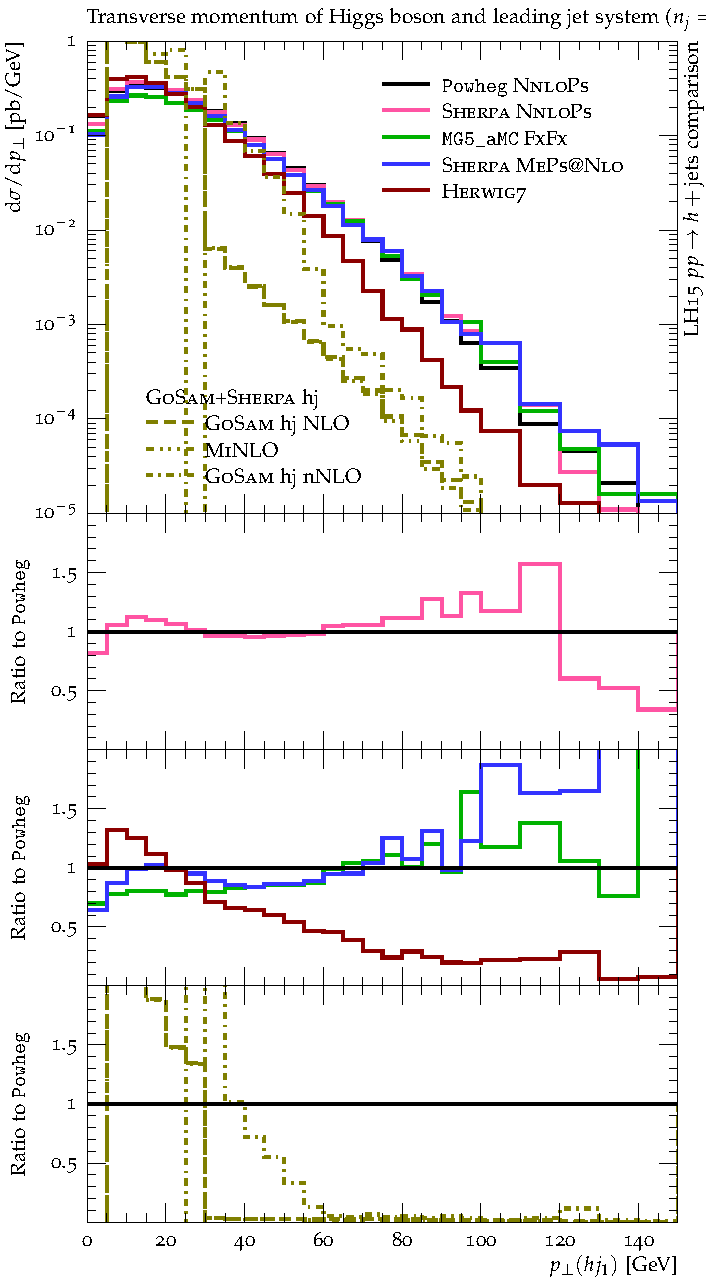
\includegraphics[width=0.47\textwidth]{figures/hjetscomp_u_Hj_pT_excl.pdf}
  \hfill
  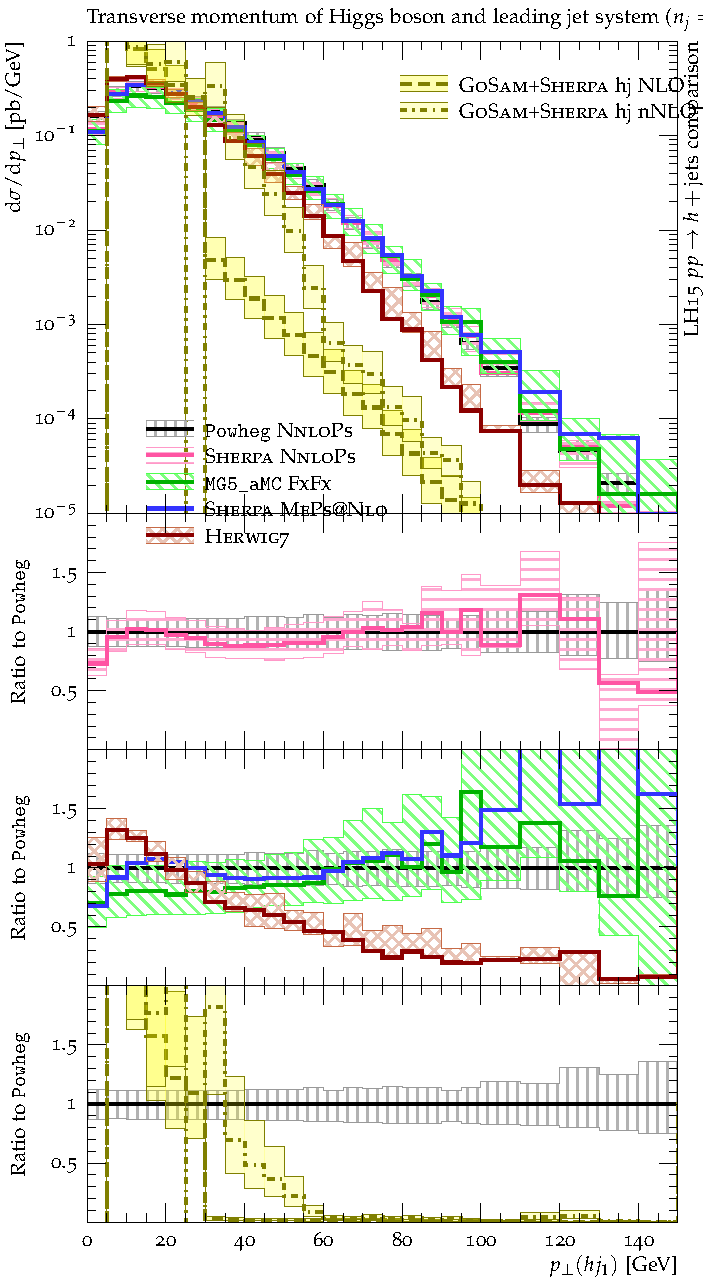
\includegraphics[width=0.47\textwidth]{figures/hjetscomp_Hj_pT_excl.pdf}
  \caption{\label{fig:hjetscomp:results:1obs:hj_pt_excl}%
    The transverse momentum of the Higgs-boson-leading-jet system in
    the presence of exactly one jet. Again, results are shown without
    (left) and with (right) theoretical uncertainties as given by the
    different groups. Note that the plot layout corresponds exactly to
    that of Figure~\ref{fig:hjetscomp:results:1obs:j1y}, except for
    the extended $\hat y$-axis range used in the ratio plots.}
\end{figure}

We finish this section by examining the results for the transverse
momentum of the Higgs-boson plus leading-jet system. In other words,
we are interested in studying the different answers in describing the
recoil of the $hj_1$ system. In the inclusive one-jet case depicted in
Figure~\ref{fig:hjetscomp:results:1obs:hj_pt}, the system may recoil
against a second jet (or secondary jets) plus soft radiation, while
for the exclusive jet scenario shown in
Figure~\ref{fig:hjetscomp:results:1obs:hj_pt_excl}, it is only soft
radiation that recoils against the $hj_1$ system. The latter case will
therefore be strongly affected by the level at which resummation is
taken into account. Formally, for the observable in question, the
predictions of highest accuracy are facilitated by the NLO merging
approaches as they provide an NLO description of the second jet; all
other predictions are only LO accurate in the second jet, i.e.~larger
differences can be expected. In the exclusive ($=1$-jet) case, all
predictions that include parton showering operate at the same level of
precision while the fixed-order calculations cannot do anything but
fail in describing the $p_\perp(hj_1)$ distribution.

For the $h\pl\ge1$-jet events, differences of $\mathcal{O}(30\%)$ are
observed among the ME+PS predictions below the jet threshold, while
there is better agreement at higher $p_\perp$ values, where again
\Herwig turns out to be on the softer side. The \Powheg curve
surprisingly fits right in with the ME+PS results, while \Sherpa's
\NNLOPS prediction only starts deviating for larger $p_\perp$ yielding
a 40\% increase at $p_\perp\sim400\gev$ (again owing to the different
treatment of scales in both approaches). The mostly comparable
behaviour of the \NNLOPS results to those obtained from NLO merging is
not what one would expect a priori, however the NNLO matching seems to
constrain the parton showers in a beneficial way (via sophisticated
choices for setting the renormalization, factorization and resummation
scales) such that the LO+PS treatment of the $h\pl\ge2$-jet rate
obtains a more appropriate normalization. The $hj$ NLO calculations
(i.e.~the pure and \Minlo reweighted \GoSam+\Sherpa results) cannot
compete with this performance since the scale setting is global and
the second-jet description is purely one of LO accuracy.
Correspondingly, the $p_\perp(hj_1)$ observable is described poorely
with values clearly overshooting below the jet threshold due to the
missing Sudakov suppression and undershooting by 60\% beyond
$p_\perp=50\gev$ due to missing higher (than two-) jet multiplicity
contributions. It is interesting to see that the \Loopsim procedure
lifts this large discrepancy in the $p_\perp$ tail. The good agreement
with the ME+PS results is largely driven by the $hjj$ NLO component
used to build the nNLO prediction for the $h\pl\ge1$ process. However,
as a result of the cut-off dependence of the procedure nothing can
be said about the $p_\perp<25\gev$ region. Lastly, we comment on the
uncertainties quoted by the different calculations: the \GoSam, \Minlo
and \Loopsim envelopes have an appropriate size reflecting the
underlying LO nature of the $p_\perp(hj_1)$ prediction above the jet
threshold, and similarly for \Sherpa's \NNLOPS result. \MGaMC and
\Herwig produce NLO variations that are fairly different in size.
However, the \Herwig as well as the \Powheg envelopes are most likely
underestimated, in particular the \Powheg band does not behave as
expected from a LO variation for above-jet-threshold $p_\perp$.

The exclusive (exactly one jet) case for describing the
$p_\perp(hj_1)$ observable is shown in
Figure~\ref{fig:hjetscomp:results:1obs:hj_pt_excl}. Apart from the
\NNLOPS outcomes, there is a much greater divergence of the
predictions for exactly one jet, especially at high $p_\perp$. Recall
this time, the recoil is generated only from soft emissions, and it is
clear that a highly exclusive distribution such as the one in question
serves as a stress test for the ME+PS as well as the \NNLOPS
predictions (in fact any parton shower or resummed prediction). For
the same reason, caution has to be taken in interpreting the shown
uncertainties. The current case is similar to the case for the Higgs
boson $p_\perp$ distribution with no jets and it is no surprise that
different approaches can lead to different answers. Most notably, we
observe \NNLOPS predictions that are in much better agreement as
compared to the inclusive case, the expected complete failure of the
\GoSam results (including the \Loopsim result where the one-jet
requirement obliterates the effect that yielded the improvement in the
inclusive case),\footnote{Owing to the kinematic constraints on the
  jets, harder radiation that goes forward does not get identified as a
  jet; these contributions actually form the (naively unexpected)
  $p_\perp>30\gev$ tail of the \GoSam results, though the mechanism is
  highly suppressed.}
and the severe decline of the \Herwig differential cross section
dropping to about 25\% wrt.~the \Powheg result at $p_\perp\sim100\gev$.

\Todo{the pT plot range of the hj1 sytem goes out to 400, in the pT
  observables before we mainly did do 200? Any opinions? pro: it's a
  system pT; contra: mainly LO, all others are 200.}



\subsection{Dijet observables}
\label{sec:hjetscomp:results:2jobs}

\Todo{similarly to previous todo: plot range of hj1j2 system goes out
  to 400, but here also for pThiggs,
  fig~\ref{fig:hjetscomp:results:2obs:hpt_j2pt}, for the latter at
  least we should go to 200 as in the other pThiggs plots}

\Todo{single-particle rapidity plots, yHiggs, yJet1, in paper have a
  [GeV] legend ... need be corrected}

\Todo{some of the plots in paper (e.g. nj, HT, veto xsecs) carry this
  vertical LH15 comparison line on their right ... extend to all plots
  in paper?}

\Todo{the gosam legend description of the no-uncertainty plots is
  different from that of the have-uncertainty plots ... the latter
  legend description looks better.}

\Todo{fig~\ref{fig:hjetscomp:results:2obs:dyjj_fb}, the DeltaY(j,j)
  using forward/backward tagging seems incomplete,
  also carries just Minlo results? Missing axis titles.}

\begin{figure}[t!]
  \centering
  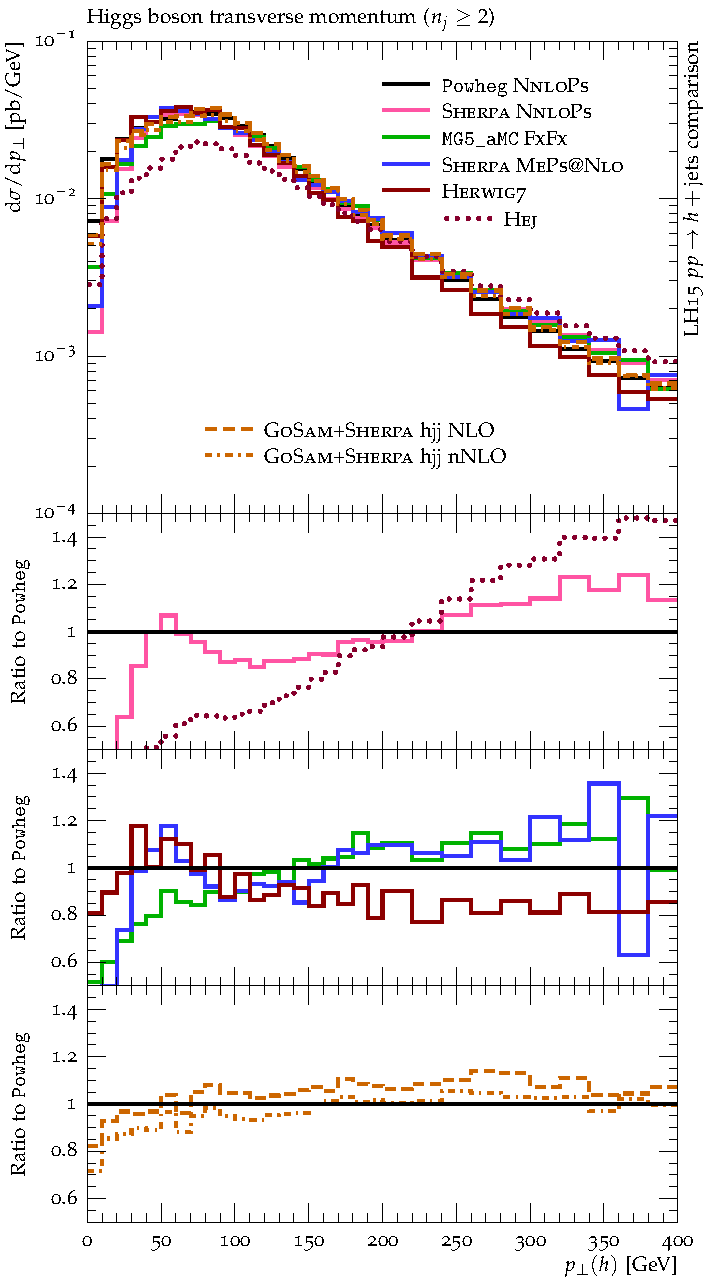
\includegraphics[width=0.47\textwidth]{figures/hjetscomp_u_H_jj_pT_incl.pdf}
  \hfill
  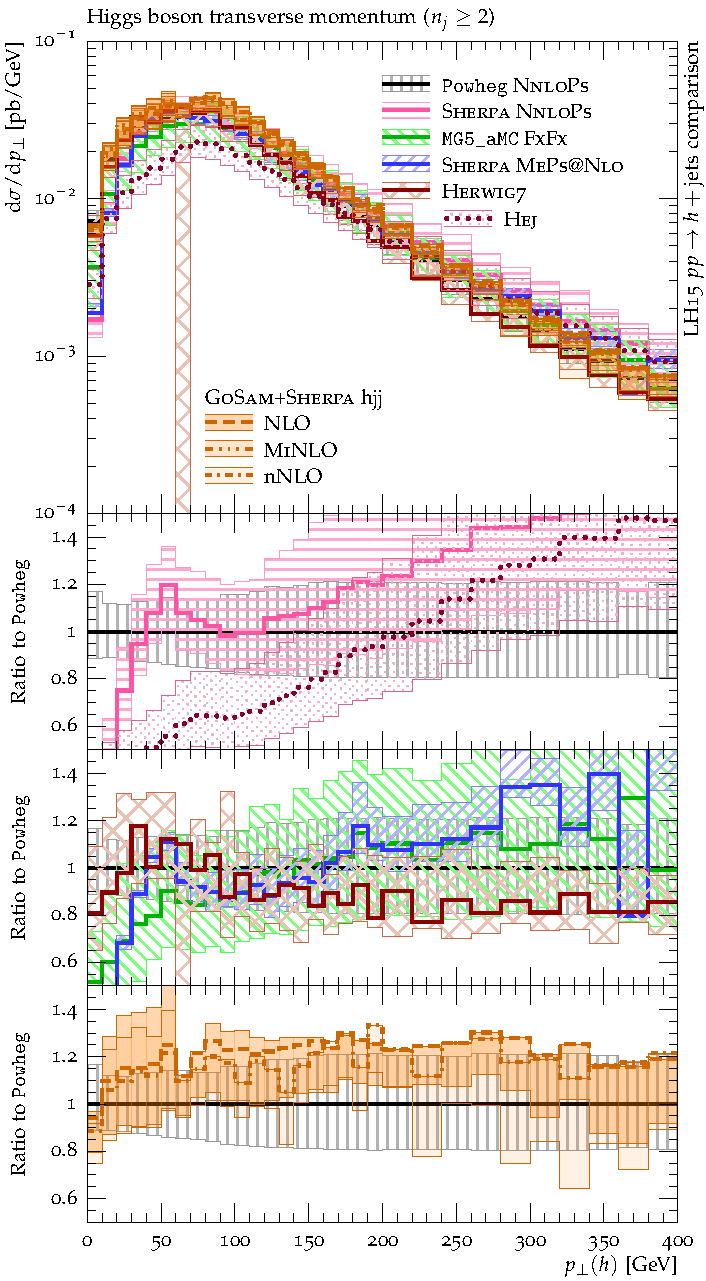
\includegraphics[width=0.47\textwidth]{figures/hjetscomp_H_jj_pT_incl.pdf}
  \caption{\label{fig:hjetscomp:results:2obs:hpt_j2pt}%
    The transverse momentum of the Higgs boson in the presence of at
    least two jets without (left) and with (right) uncertainties,
    supplemented by three ratio plots using the reference result as
    obtained from \Powheg's \NNLOPS calculation for $h$ production.
    The predictions are grouped -- from top to bottom -- according to
    the categories \NNLOPS $h$ production, ME+PS merging at NLO (at
    least up to two jets) and NLO fixed-order $hjj$ production. \Hej's
    prediction is added to the first, the \NNLOPS, subpanel.}
\end{figure}

The Higgs boson $p_T$, in the presence of at least two jets, is shown
in Figure~\ref{fig:hjetscomp:results:2obs:hpt_j2pt}. Here, varying
behavior is observed, with MG5 and Sherpa being substantially lower
than Powheg at low $p_T$ and somewhat higher at high $p_T$, while
Herwig7 is somewhat lower than Powheg at high $p_T$. The gosam
$H+\ge2$ jet prediction is lower than Powheg at low $p_T$ (as expected
for a Sudakov region),and roughly 10\% higher at high $p_T$ (closer to
the MG5/Sherpa predictions).

\begin{figure}[t!]
  \centering
  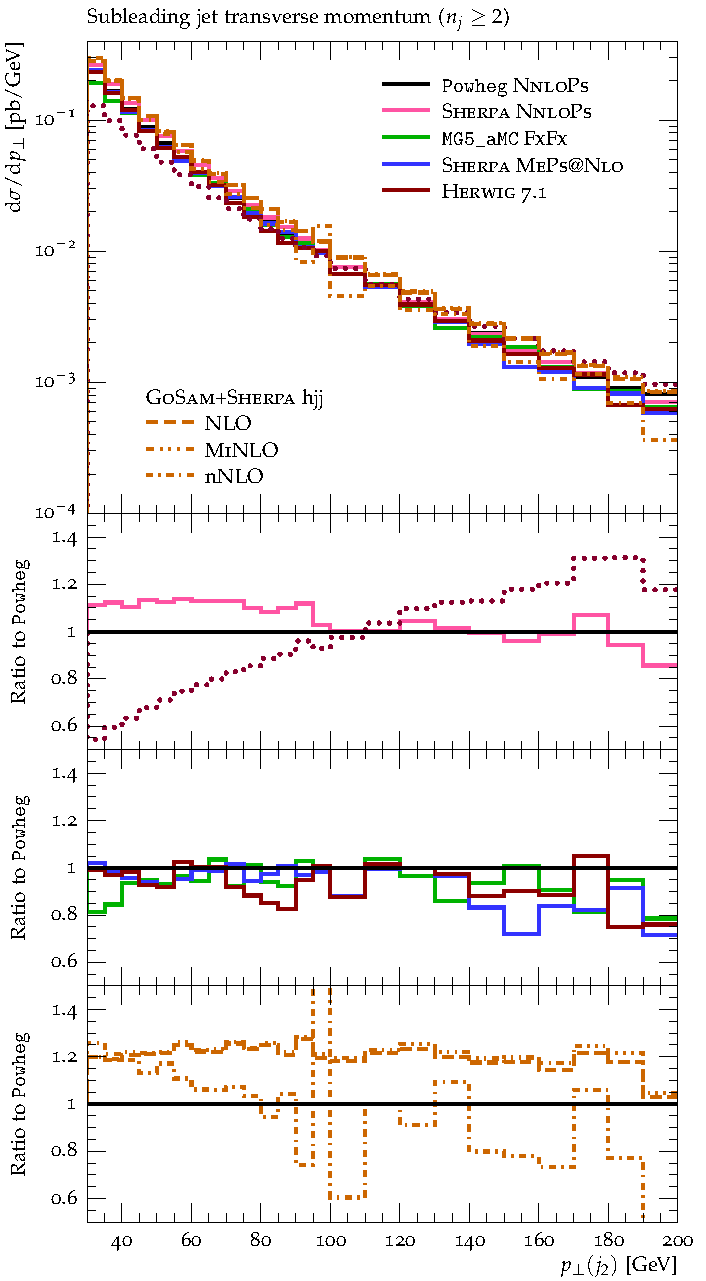
\includegraphics[width=0.47\textwidth]{figures/hjetscomp_u_jet2_pT_incl.pdf}
  \hfill
  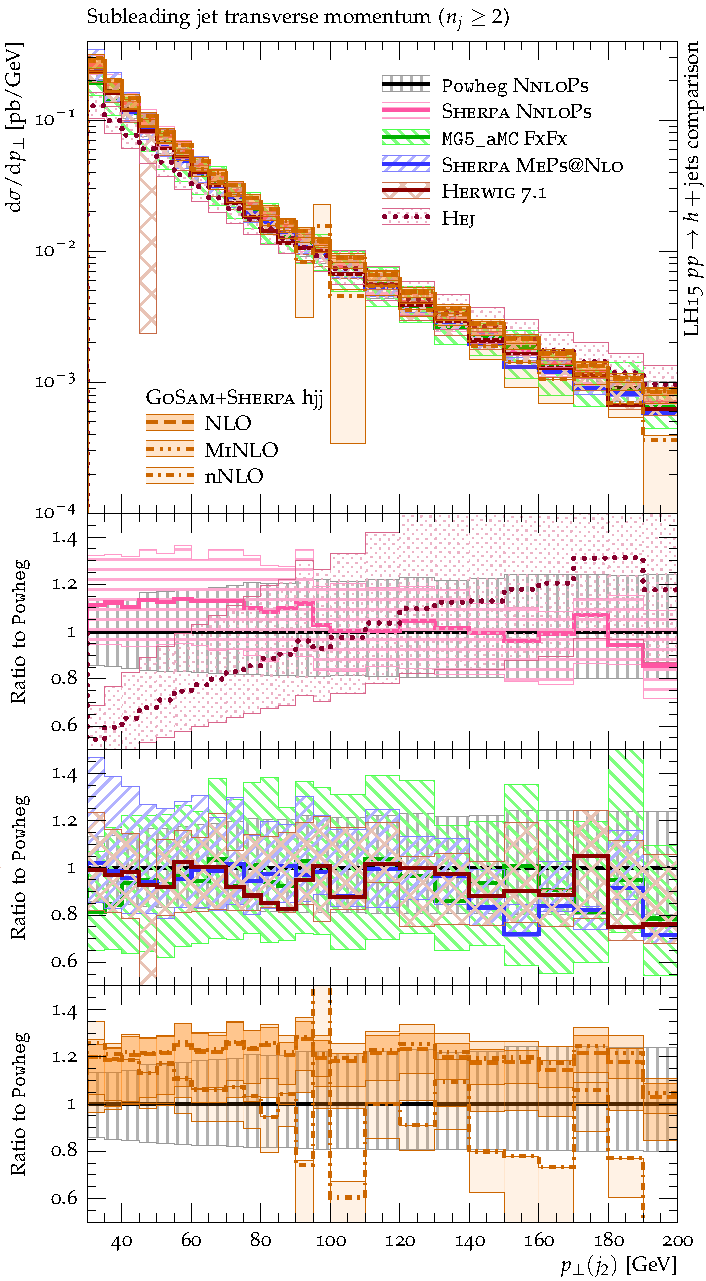
\includegraphics[width=0.47\textwidth]{figures/hjetscomp_jet2_pT_incl.pdf}
  \caption{\label{fig:hjetscomp:results:2obs:jet2_pt}%
    The subleading jet $p_\perp$ for $h\pl\ge2$-jets production shown
    without (left) and with (right) theoretical uncertainties. The
    plot layout is the same as in the previous figure.}
\end{figure}

\begin{figure}[t!]
  \centering
  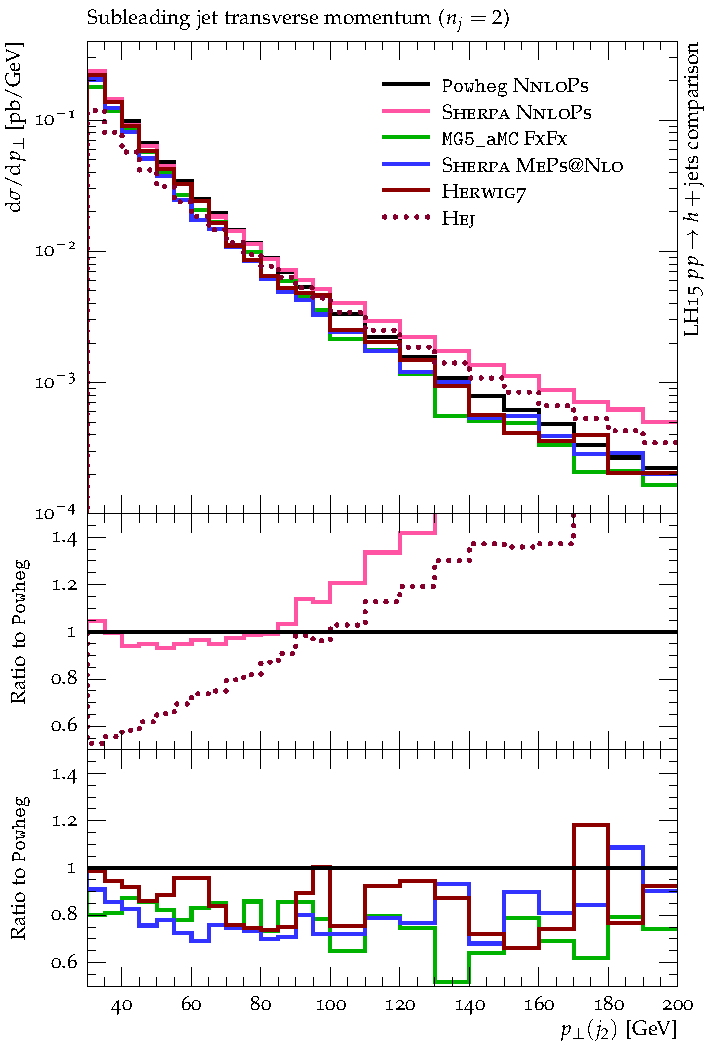
\includegraphics[width=0.47\textwidth]{figures/hjetscomp_u_jet2_pT_excl.pdf}
  \hfill
  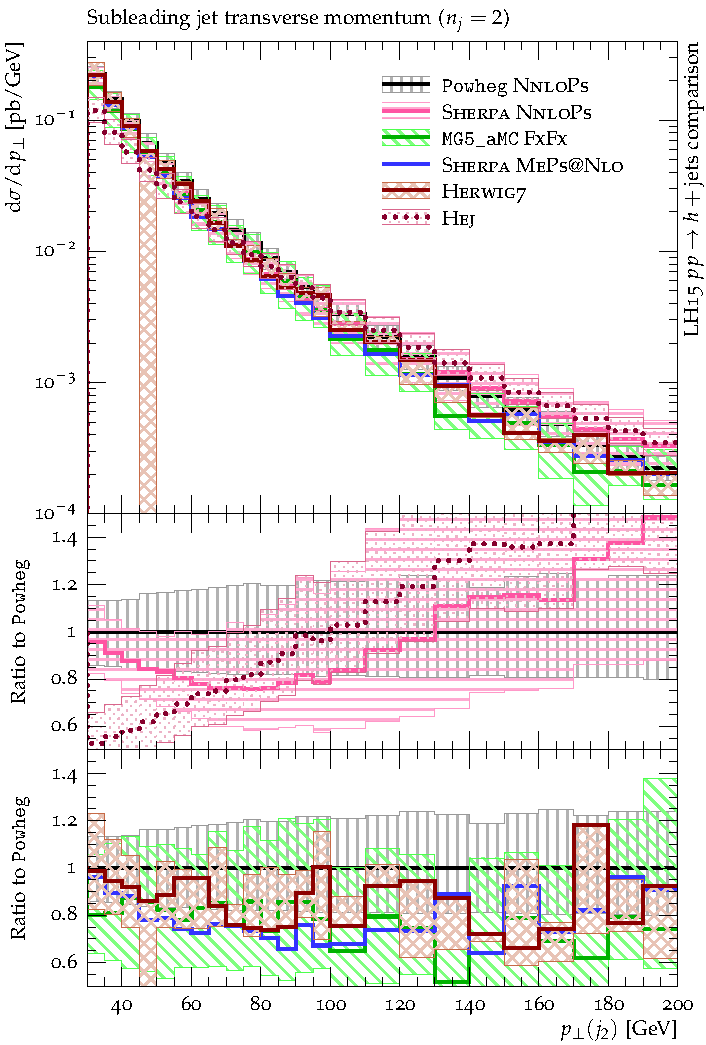
\includegraphics[width=0.47\textwidth]{figures/hjetscomp_jet2_pT_excl.pdf}
  \caption{\label{fig:hjetscomp:results:2obs:jet2_pt}%
    The subleading jet $p_\perp$ for exclusive $h\pl2$-jets production
    shown without (left) and with (right) theoretical uncertainties.
    Again, the layout is similar to that of
    Figure~\ref{fig:hjetscomp:results:2obs:hpt_j2pt} except for
    dropping the results of the NLO fixed-order $hjj$ production and
    the associated ratio subpanel.}
\end{figure}

The sub-leading jet $p_T$ for $H+\ge2$ jets is shown in the upper row
of Figure~\ref{fig:hjetscomp:results:2obs:jet2_pt}.  The agreement
among the ME+PS predictions and between the ME+PS and fixed order
predictions of gosam is better than in the case of the leading
jets. With two or more jets in the final state, meaningful predictions
to HEJ can be made for the first time.

The sub-leading jet $p_T$ for $H$ + exactly 2 jets is shown in the
lower panel of Figure~\ref{fig:hjetscomp:results:2obs:jet2_pt}.
Here, MG5, Sherpa and Herwig7 lie in reasonable agreement with each
other, but systematically lower than Powheg.

\Todo{physics?}

\begin{figure}[t!]
  \centering
  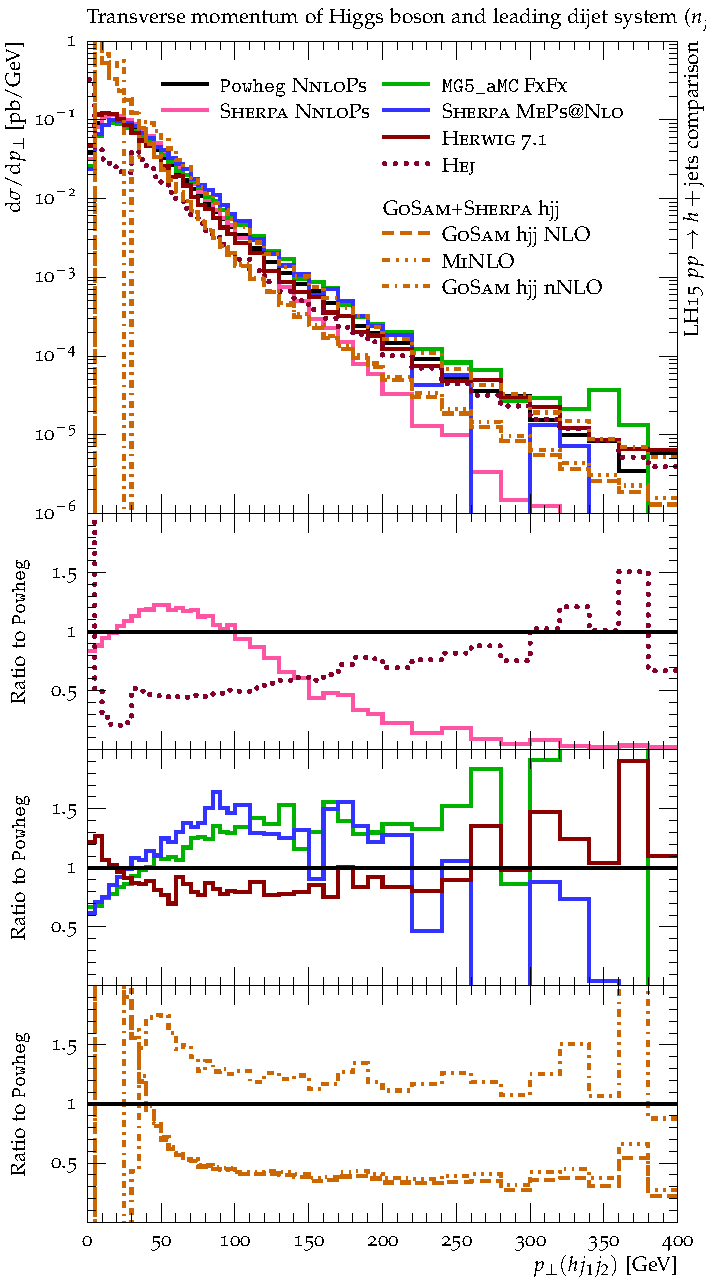
\includegraphics[width=0.47\textwidth]{figures/hjetscomp_u_Hjj_pT_incl.pdf}
  \hfill
  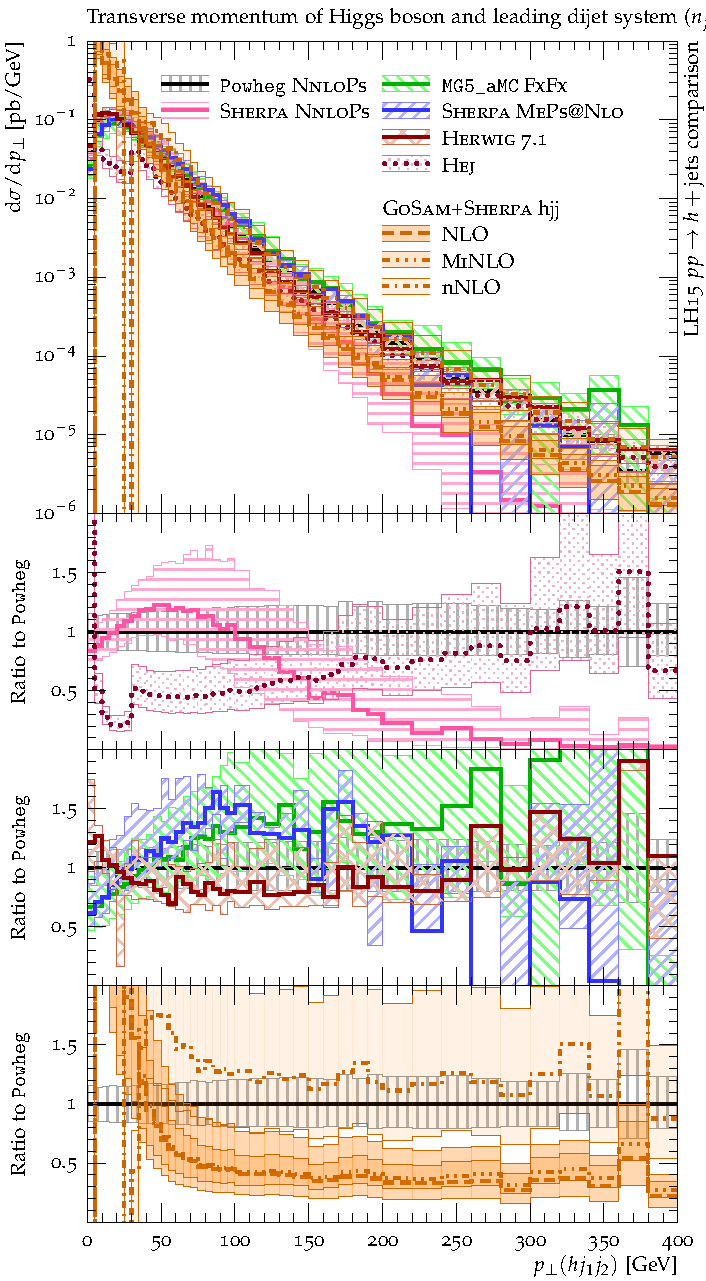
\includegraphics[width=0.47\textwidth]{figures/hjetscomp_Hjj_pT_incl.pdf}
  \caption{
    The transverse momentum of the Higgs boson plus two leading jet
    system without (left) and with (right) uncertainties.
    \label{fig:hjetscomp:results:2obs:hjj_pt}
  }
\end{figure}

The transverse momentum of the Higgs boson plus two leading jet system
is shown in Figure~\ref{fig:hjetscomp:results:2obs:hjj_pt}. Varying
behavior is also observed here, with MG5 and Sherpa being having a
slope with respect to Powheg at low $p_T$ and being somewhat higher at
high $p_T$, while Herwig7 is again somewhat lower than Powheg at high
$p_T$. The gosam $H+\ge2$ jet prediction is much higher than Powheg at
low $p_T$, and significantly lower at high $p_T$.

\Todo{physics!; why does gosam have the behavior it does?}

\begin{figure}[t!]
  \centering
  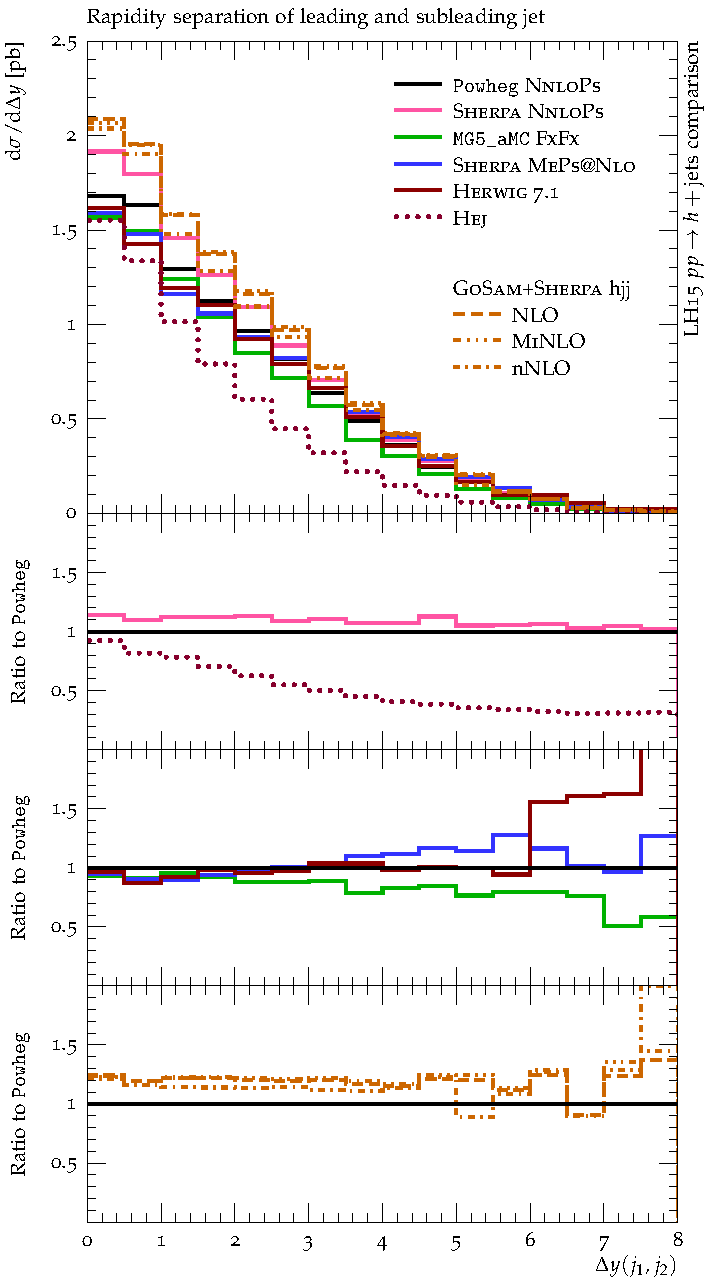
\includegraphics[width=0.47\textwidth]{figures/hjetscomp_u_deltay_jj.pdf}
  \hfill
  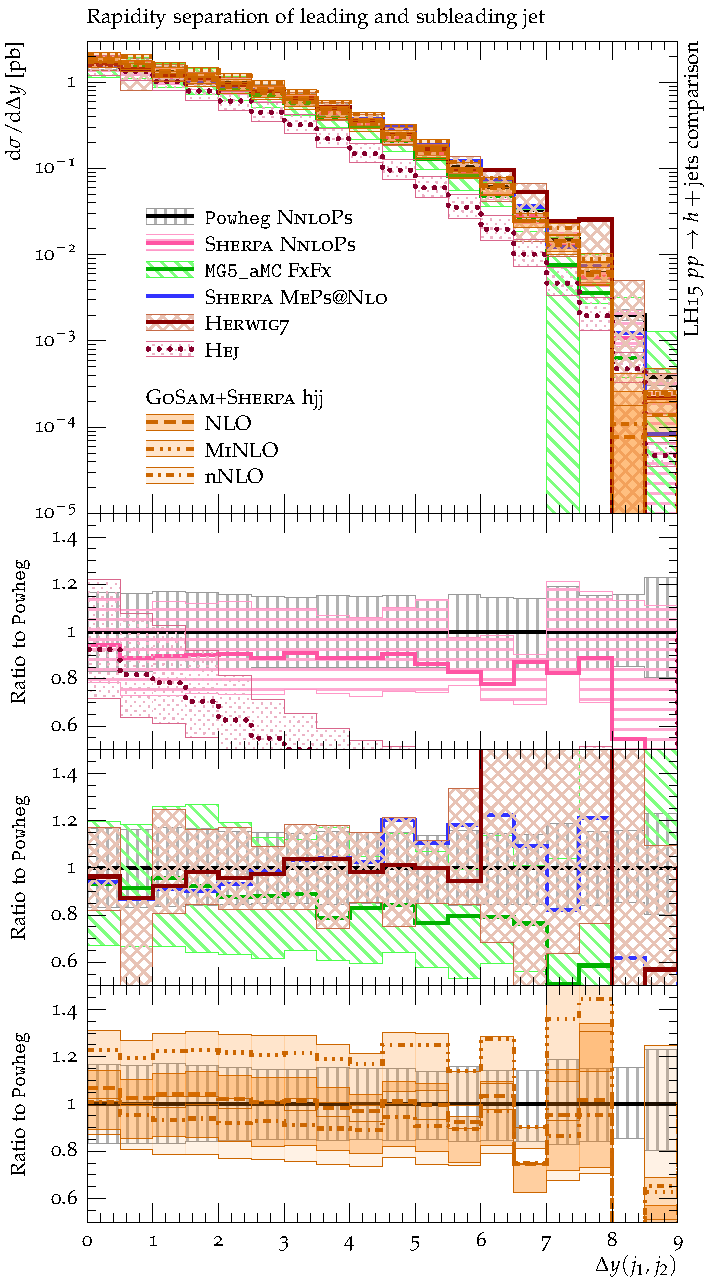
\includegraphics[width=0.47\textwidth]{figures/hjetscomp_deltay_jj.pdf}
  \caption{
    The rapidity separation between the leading and sub-leading jets
    for $H+\ge2$ jets, without (left) and with (right) uncertainties.
    \label{fig:hjetscomp:results:2obs:dyjj}
  }
\end{figure}

\begin{figure}[t!]
  \centering
  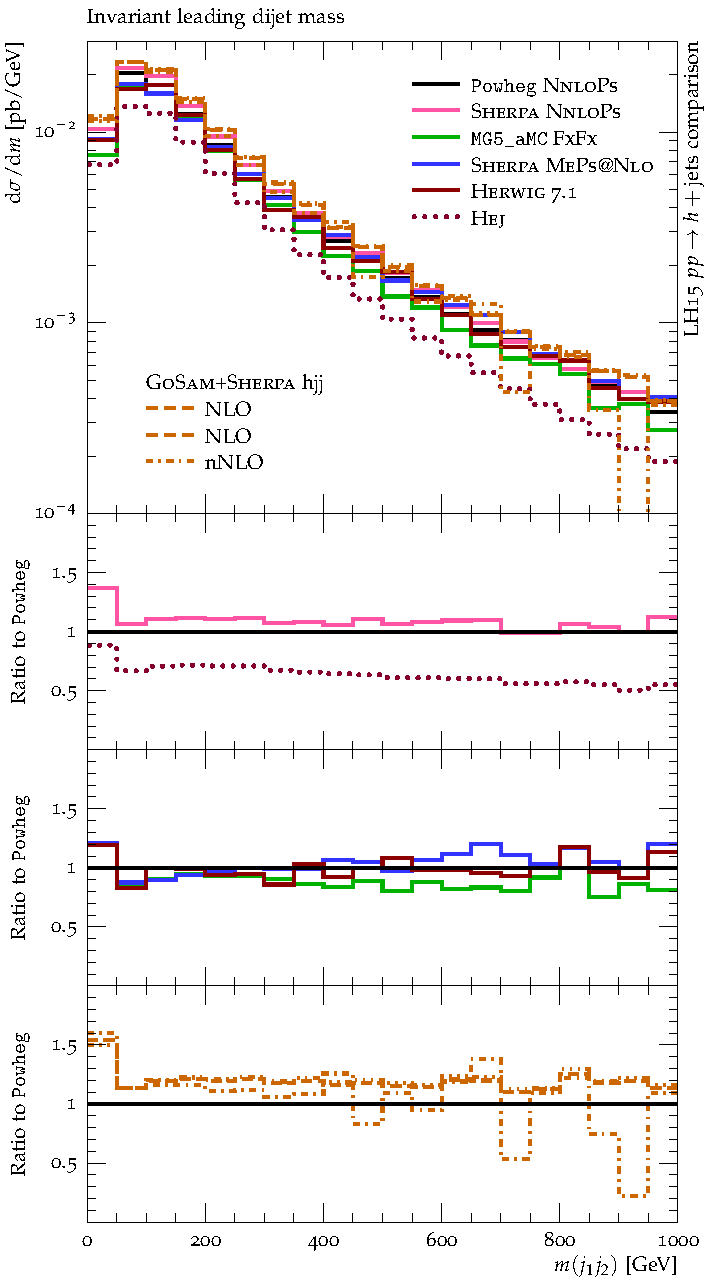
\includegraphics[width=0.47\textwidth]{figures/hjetscomp_u_dijet_mass.pdf}
  \hfill
  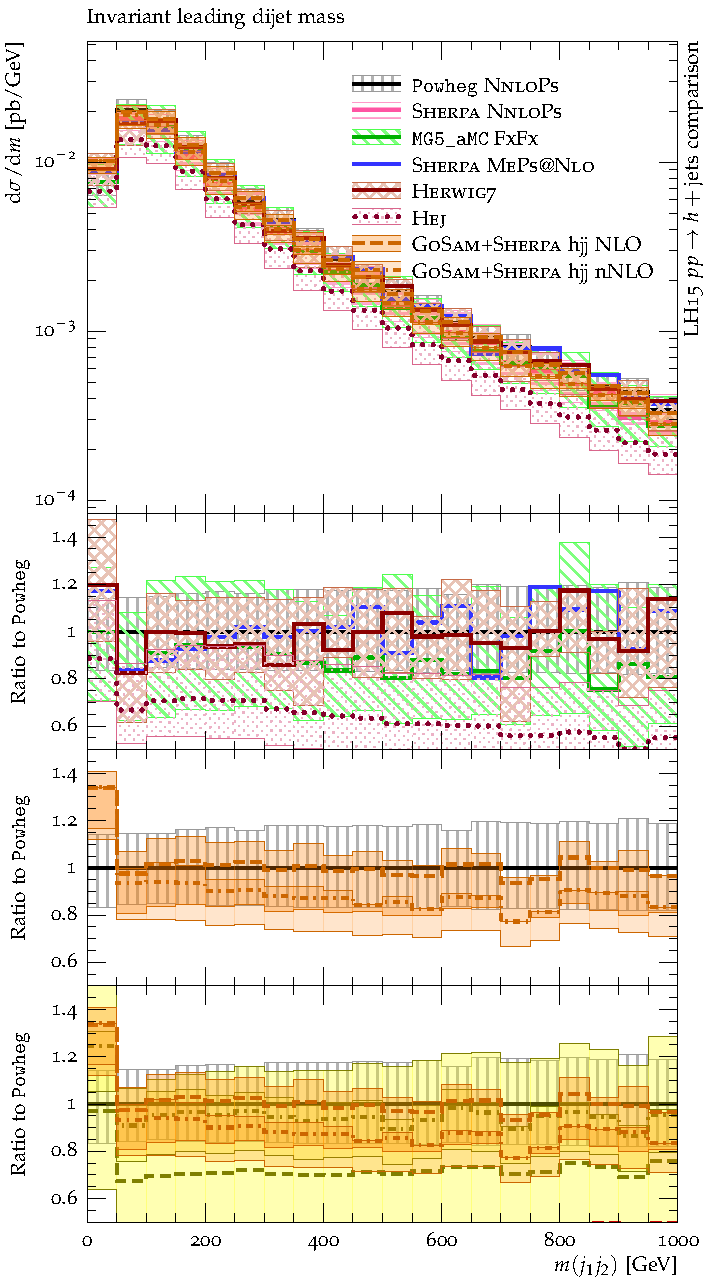
\includegraphics[width=0.47\textwidth]{figures/hjetscomp_dijet_mass.pdf}
  \caption{
    The invariant mass of the leading dijet system without (left) and
    with (right) uncertainties.
    \label{fig:hjetscomp:results:2obs:mjj}
  }
\end{figure}

The rapidity separation between the leading and sub-leading jets is
shown in Figure~\ref{fig:hjetscomp:results:2obs:dyjj}, for $H+\ge2$
jets. MG5 is lower than Powheg at high $\Delta y$ (while Sherpa is
slightly higher).  Powheg is in good agreement with the fixed order
gosam results for $H+\ge2$ jets. Similar conclusions hold for for the
dijet mass distribution, as shown in
Figure~\ref{fig:hjetscomp:results:2obs:mjj}, although the differences
among predictions are smaller.

\begin{figure}[t!]
  \centering
  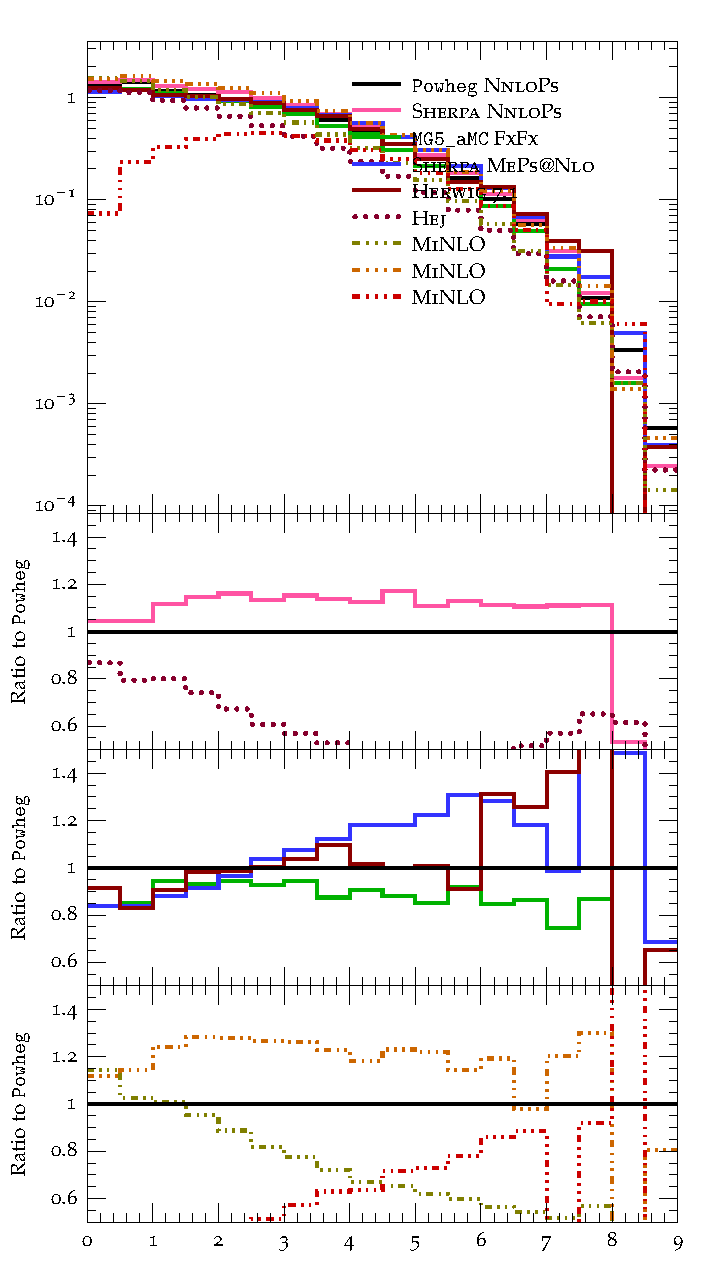
\includegraphics[width=0.47\textwidth]{figures/hjetscomp_u_jjfb_dy.pdf}
  \hfill
  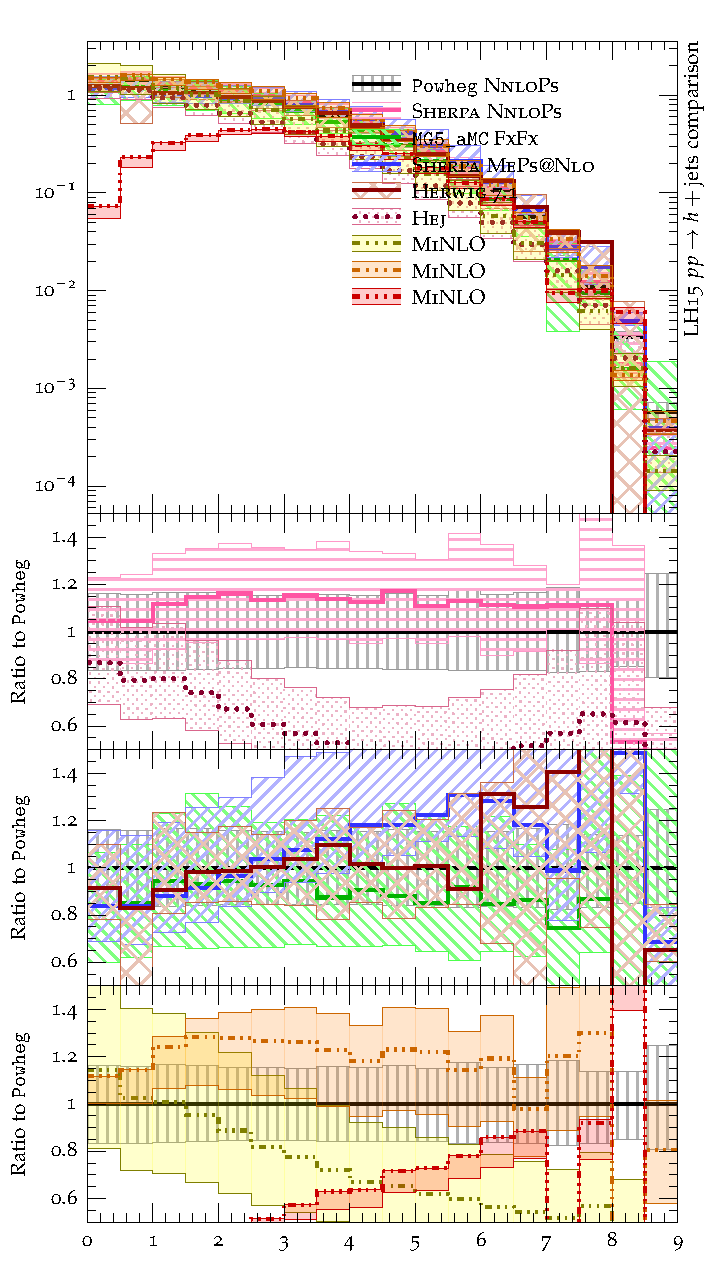
\includegraphics[width=0.47\textwidth]{figures/hjetscomp_jjfb_dy.pdf}
  \caption{
    The rapidity separation between the two most forward-backward jets
    for $H+\ge2$ jets, without (left) and with (right) uncertainties. 
    \label{fig:hjetscomp:results:2obs:dyjj_fb}
  }
\end{figure}

The rapidity separation between the two most forward-backward jets is
shown in Figure~\ref{fig:hjetscomp:results:2obs:dyjj_fb}. As for the
$p_T$-ordered distribution, MG5 is lower than Powheg at high $\Delta
y$ while Sherpa is higher. Powheg now has a slope compared to the
Gosam NLO results, but, interestingly, not compared to the nNLO
results.

\begin{figure}[t!]
  \centering
  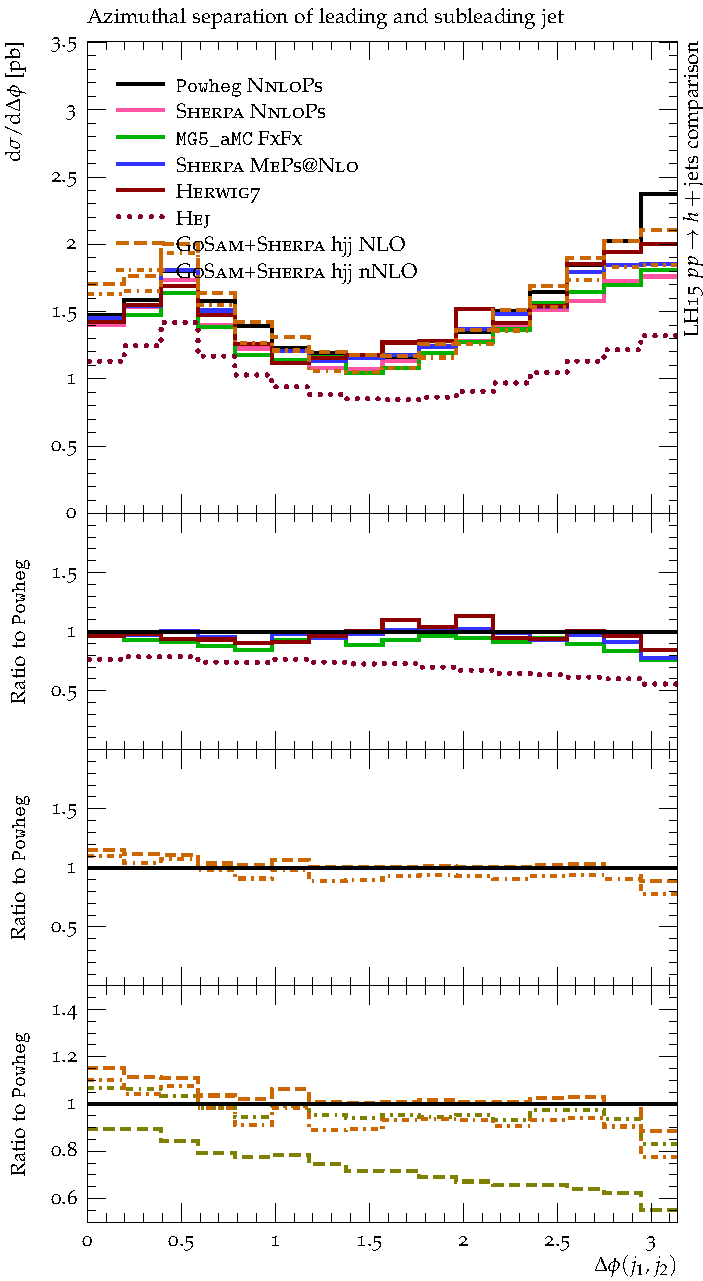
\includegraphics[width=0.47\textwidth]{figures/hjetscomp_u_deltaphi_jj_incl.pdf}
  \hfill
  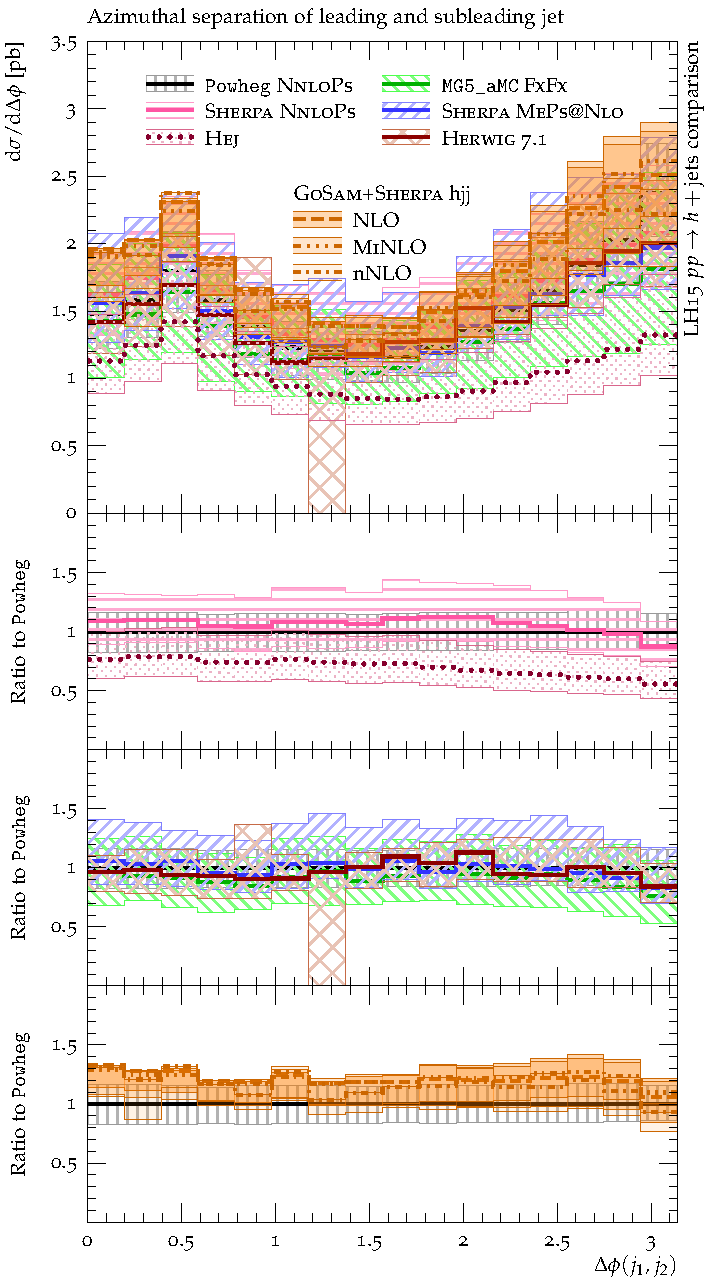
\includegraphics[width=0.47\textwidth]{figures/hjetscomp_deltaphi_jj_incl.pdf}
  \caption{
    The $\Delta\phi$ separation between the two leading jets for
    $H+\ge2$ jets, without (left) and with (right) uncertainties. 
    \label{fig:hjetscomp:results:2obs:dphi_jj}
  }
\end{figure}

The $\Delta\phi$ separation between the two leading jets is shown in
Figure~\ref{fig:hjetscomp:results:2obs:dphi_jj}. All predictions are
in good agreement with each other, except for HEJ, which has a leading
order normalization. Similar distributions (and agreement) are
observed if the two most forward-backward jets are chosen instead.



\clearpage
\subsection{VBF observables}
\label{sec:hjetscomp:results:VBFobs}

A situation where Higgs production in gluon fusion primarily serves 
as background is found in analyses where its couplings to weak 
vector bosons are measured. To enhance the relative contribution 
of processes where the Higgs production proceeds through weak vector 
boson fusion (VBF) additional cuts are placed on the so-called tagging 
jets. The tagging jets themselves can now be defined in multiple ways. 
In the study performed during the Les Houches 2013 workshop 
\cite{AlcarazMaestre:2012vp} the standard leading ($p_\perp$-ordered) jet 
selection was supplemented with the forward-backward selection defining 
the pair of jets with the largest rapidity separation as tagging jets. 
Alternatives using the highest invariant mass pair were also studied 
\cite{Greiner:2015jha}. In the present study, we generalised these 
definitions, defining the tagging jets as the leading pair of 
$p_\perp$-ordered jets which fulfils the thereupon applied cuts. 
Of course, differences between the schemes only manifest themselves in 
the presence of at least three jets and are, thus, formally of higher 
order. Numerically, however, they can have a major impact and their 
choice depends on the physics aims of the analysis to be performed. 

In our analysis, requiring the tagging jet invariant mass and rapidity 
separation to be in excess of $400\,\gev$ and $2.8$, respectively, 
prepares the typical VBF kinematics. Now, the contamination of these 
observables with the irreducible background of Higgs produced in gluon 
fusion is a key quantity in the accuracy of the extraction of the coupling 
parameters. We thus proceed to analyse the congruence of the different 
descriptions of a selection of key observables with the standard tagging 
jet using the leading and sub-leading $p_\perp$-ordered jets. Results 
for the alternative choice can be found at \cite{webpage}.

\begin{figure}[t!]
  \centering
  \begin{minipage}{0.47\textwidth}
    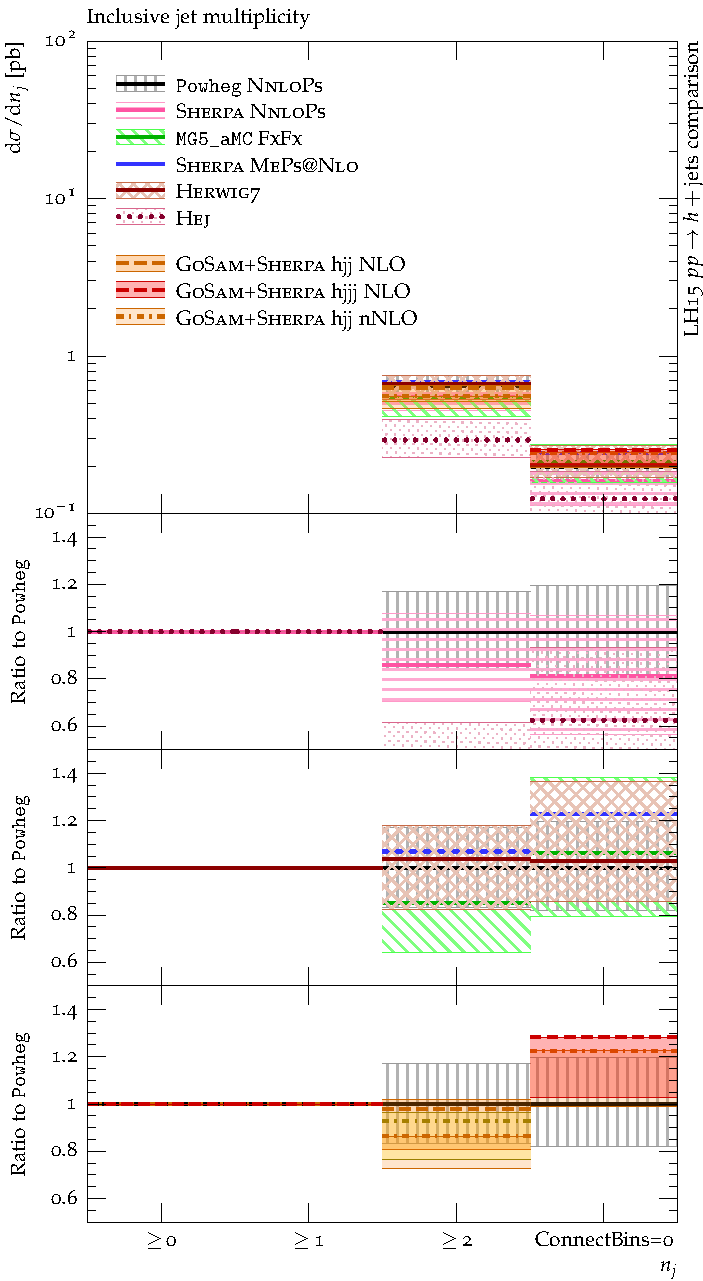
\includegraphics[width=\textwidth]{figures/hjetscomp_NJet_incl_30_VBF.pdf}
  \end{minipage}
  \hfill
  \begin{minipage}{0.47\textwidth}
    \lineskip-1.35pt
    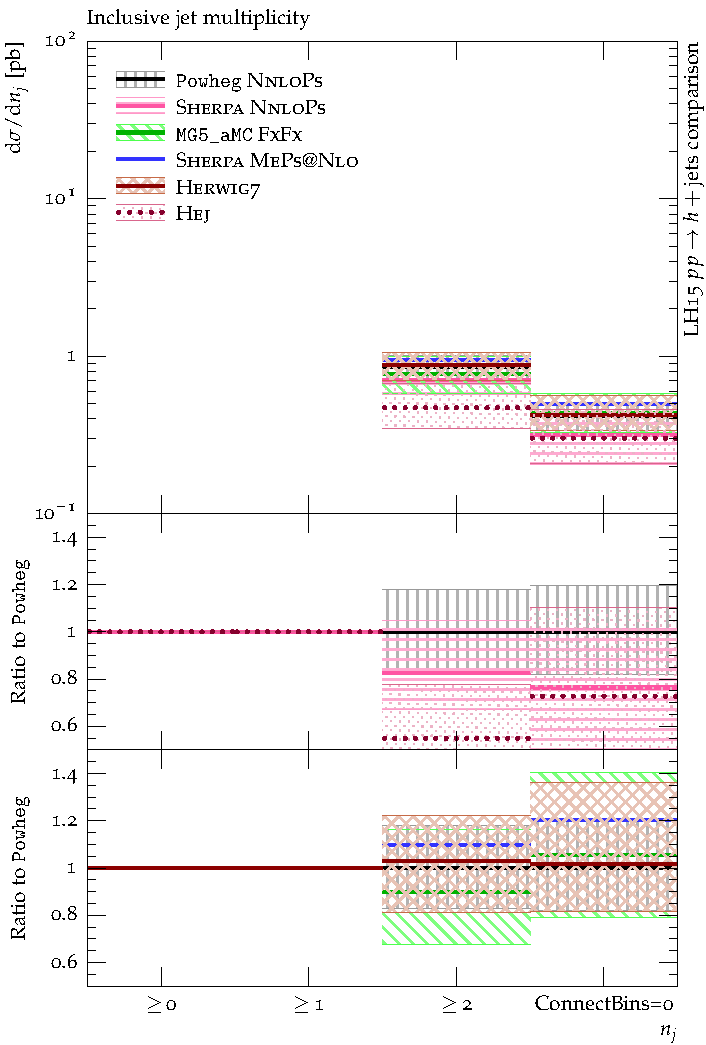
\includegraphics[width=\textwidth]{figures/hjetscomp_NJet_incl_30_VBF2.pdf}\\
    
\includegraphics[width=\textwidth]{figures/ratiopanelplaceholder.pdf}
  \end{minipage}
  \caption{
    The inclusive jet multiplicities after the application of the VBF 
    cuts standard leading tagjet definition (VBF, left) and 
    the generalised leading tagjet definition (VBF2, right).
    \label{fig:hjetscomp:results:inclobs:njets_VBF}
  }
\end{figure}

We start by examining the inclusive jet multiplicity distributions after 
the application of the above detailed VBF cuts in 
Figure~\ref{fig:hjetscomp:results:inclobs:njets_VBF}. The hierarchy
is essentially the same as for the inclusive jet multiplicity
distribution without any cuts. The differences among the predictions
are somewhat smaller with the VBF2 cuts than with the VBF cuts. 
In both cases, the \NNLOPS calculations are again in very good agreement 
with \Sherpa \NNLOPS allowing for a larger uncertainty which is driven 
by the partially evaluated resummation uncertainty not assessed in \Powheg. 
\Hej throughout predicts only about 50\% of the cross section of the the 
\NNLOPS predicted cross section. Comparing with the inclusive dijet 
cross sections of Figure \ref{fig:hjetscomp:results:inclobs:njets}
Nonetheless, the number of gluon fusion events passing the VBF 
selection criteria it therefore predicts a significantly smaller 
VBF cut efficiency. The NLO merged predictions vary from a 20\% 
smaller number of events (\MGaMC) to a 20\% larger number of events 
(\Sherpa \MEPSatNLO) surviving the event selection, both at the edge of 
the \NNLOPS uncertainty band. Interestingly, their uncertainty is of 
similar size as the \NNLOPS on, $\sim$20\%, despite being of NLO 
accuracy for these observables (only LO for \NNLOPS). This hints 
at the underestimated uncertainties of the \NNLOPS calculations for 
this observable. The NLO and \Minlo \GoSam{}+\Sherpa calculations are 
also 20\% larger than the \NNLOPS result, close to the \Sherpa \MEPSatNLO 
prediction, while the \Loopsim prediction exceeds the \NNLOPS ones only 
by about 5\%. Their uncertainties are all one-sided and with about 20\% 
of the same relative size as the NLO multijet merged uncertainties. 
Requiring a third jet sees the \NNLOPS calculations drop with respect to 
all other ones due to their thrid jet desription coming entirely from 
their parton showers' soft-collinear approximation. Otherwise, the 
picture remains unchanged. The fixed-order cross-section again is in 
rough agreement with the \Sherpa \MEPSatNLO one, their uncertainties,
however, manifesting themselves differently.

\begin{figure}[t!]
  \centering
  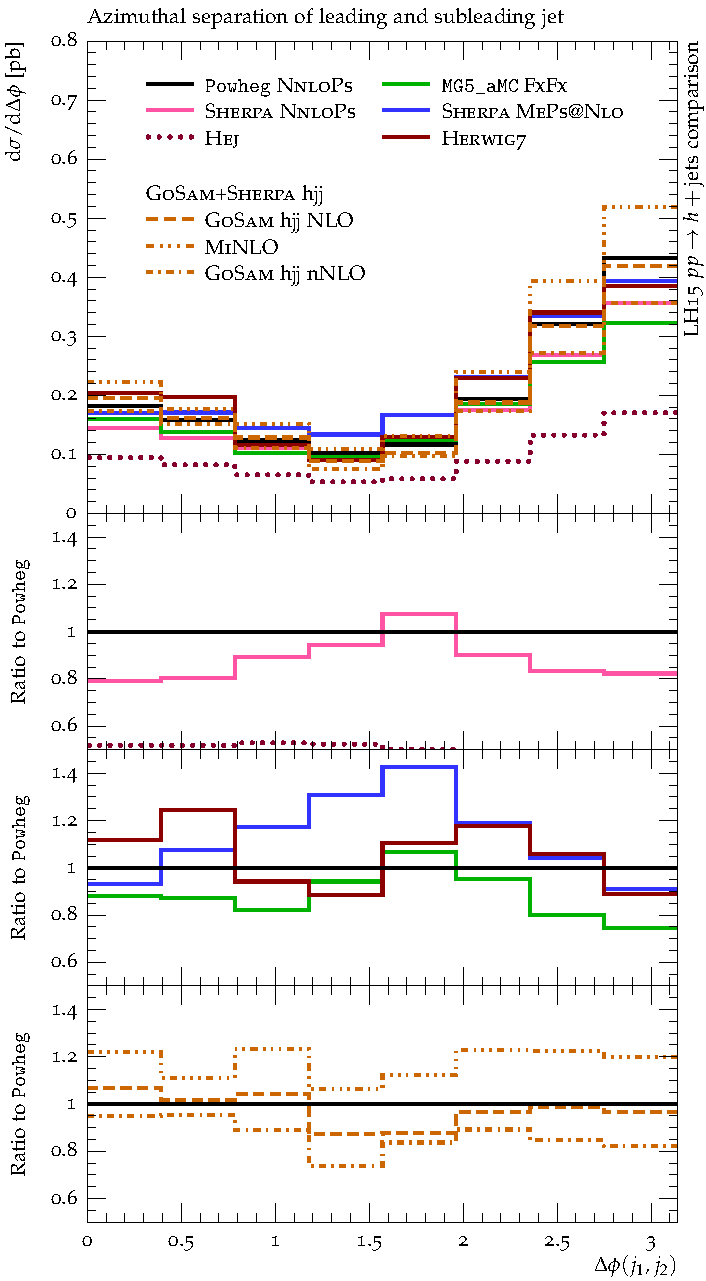
\includegraphics[width=0.47\textwidth]{figures/hjetscomp_u_deltaphi_jj_VBF.pdf}
  \hfill
  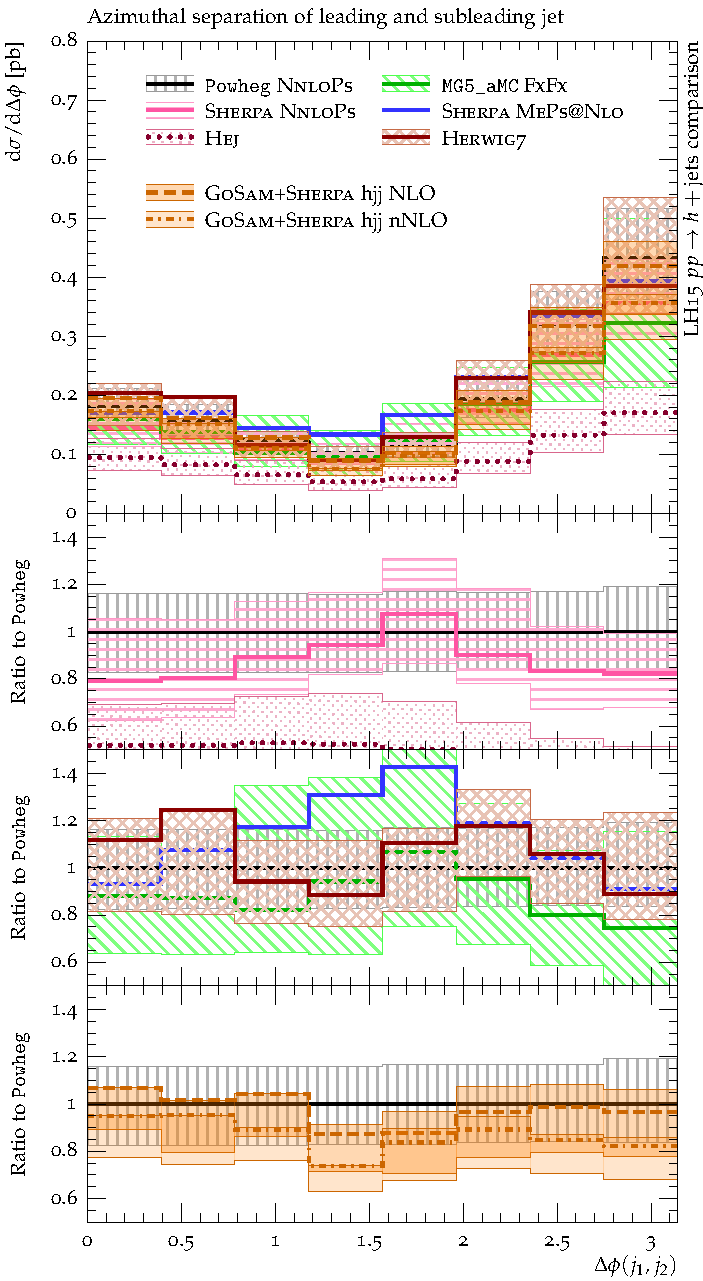
\includegraphics[width=0.47\textwidth]{figures/hjetscomp_deltaphi_jj_VBF.pdf}
  \caption{
    Azimuthal separation of the leading jet pair (left) and 
    $\Delta\phi_2$ (right) after applying VBF cuts in $H+\ge2$ jet
    production.
    \label{fig:hjetscomp:results:VBFobs:dphijj}
  }
\end{figure}

The $\Delta\phi$ separation between the two leading jets is a crucial 
observable in the VBF measurements. Its gluon fusion contribution is 
similarly described by all calculations with the uncertainties being 
$\sim$20\% throughout. Noteworthy is only the fact that \Sherpa, both 
its \NNLOPS and its \MEPSatNLO calculations, predict a shallower dip 
at $\Delta\phi(j_1,j_2)\approx\tfrac{\pi}{2}$, a fact that can be 
traced to its parton shower. Similar distributions (and agreement) 
are observed if the generalised tagging jet definition is used.

\begin{figure}[t!]
  \centering
  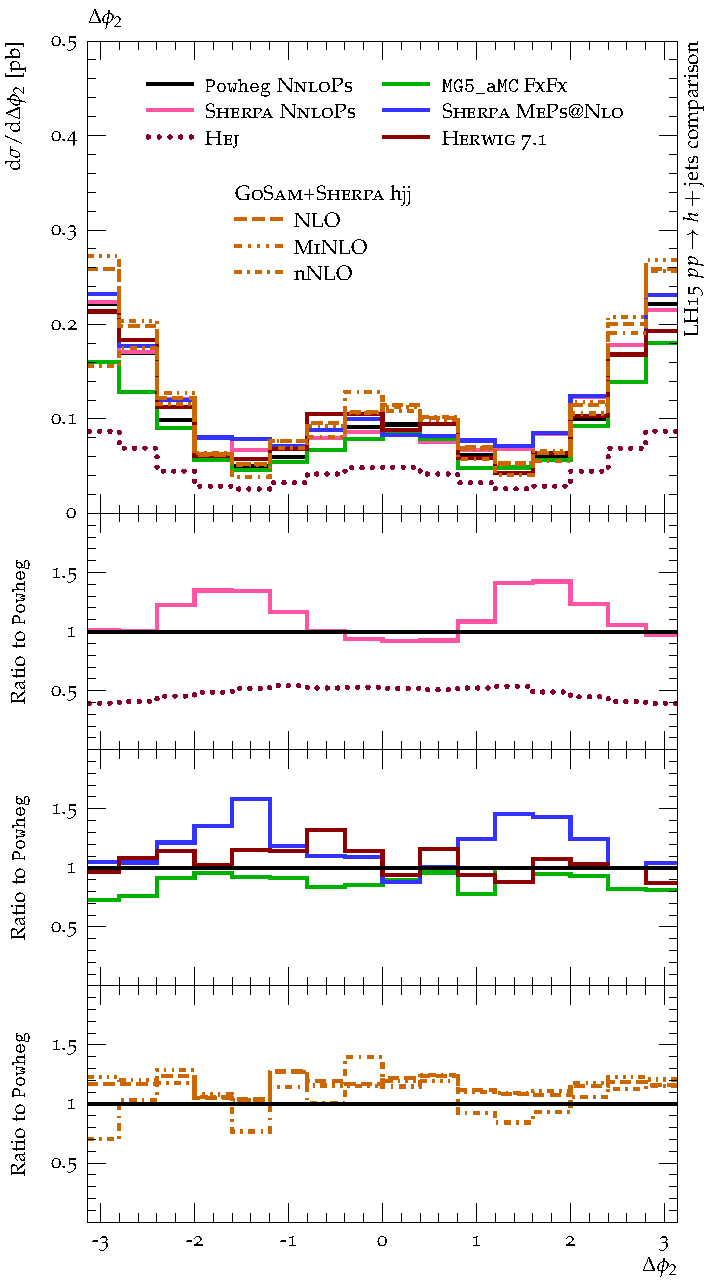
\includegraphics[width=0.47\textwidth]{figures/hjetscomp_u_deltaphi2_VBF.pdf}
  \hfill
  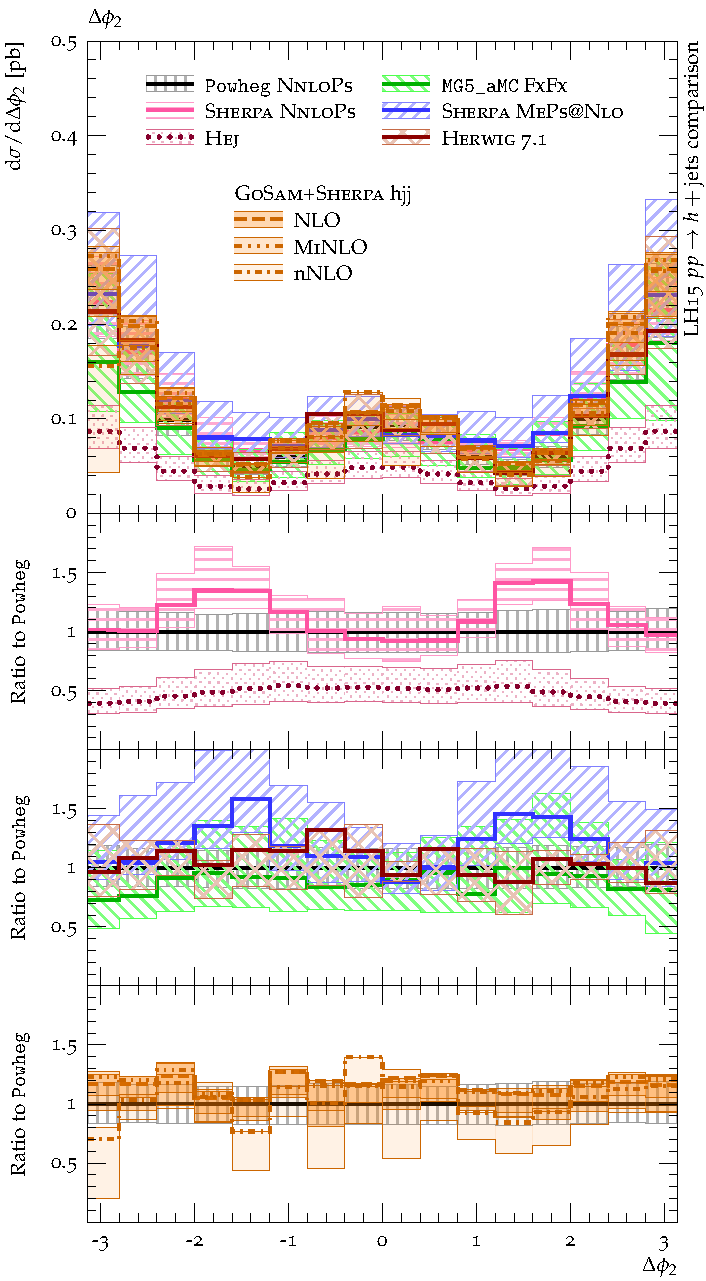
\includegraphics[width=0.47\textwidth]{figures/hjetscomp_deltaphi2_VBF.pdf}
  \caption{
    Azimuthal separation of the leading jet pair (left) and 
    $\Delta\phi_2$ (right) after applying VBF cuts in $H+\ge2$ jet
    production.
    \label{fig:hjetscomp:results:VBFobs:phi2}
  }
\end{figure}

$\Delta\phi_2$ 



\clearpage
\subsection{Multijet observables}
\label{sec:hjetscomp:results:mjobs}

\begin{figure}[t!]
  \centering
  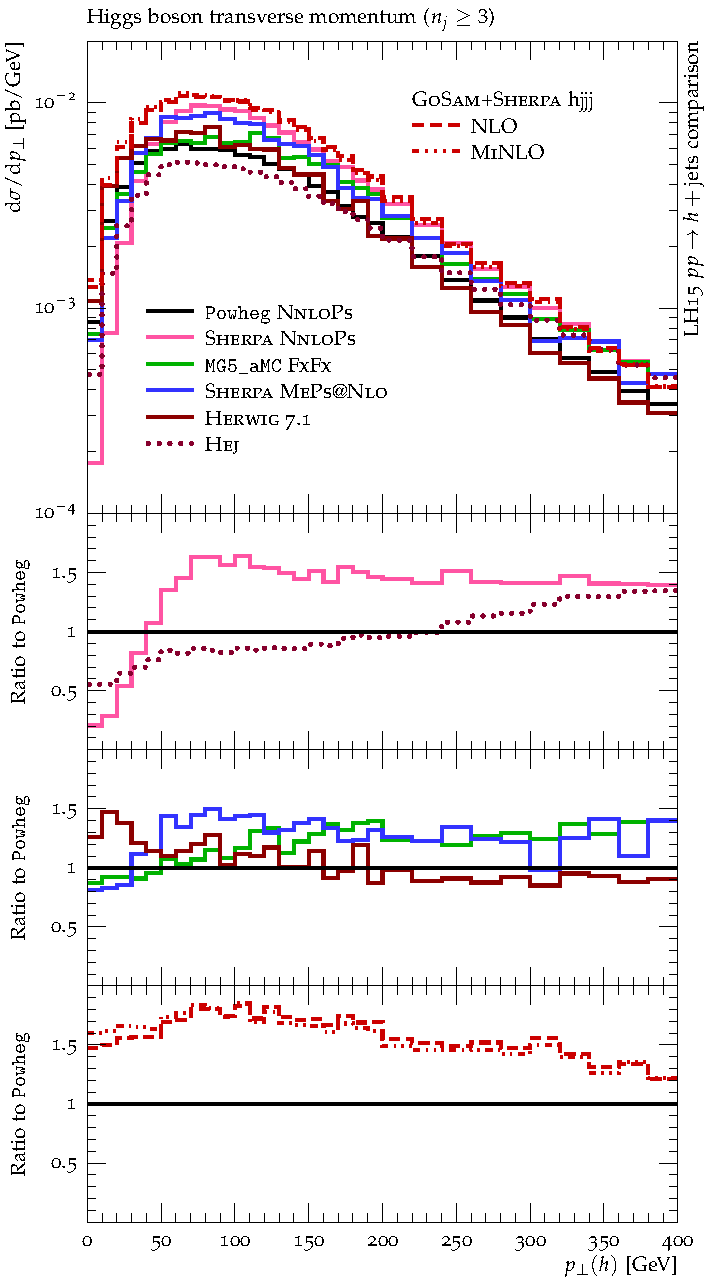
\includegraphics[width=0.47\textwidth]{figures/hjetscomp_u_H_jjj_pT_incl.pdf}
  \hfill
  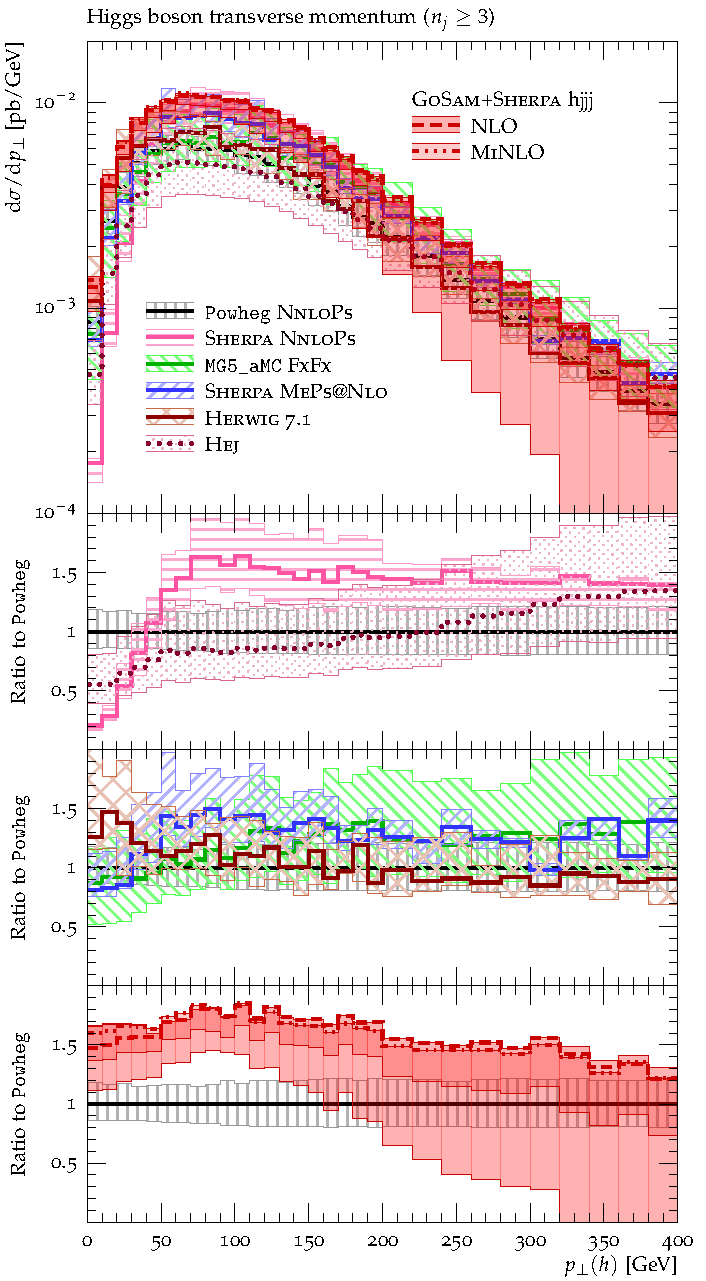
\includegraphics[width=0.47\textwidth]{figures/hjetscomp_H_jjj_pT_incl.pdf}
  \caption{
    The Higgs boson transverse momentum in the presence of at least three 
    jets, shown without (left) and with (right) theoretical uncertainties.
    \label{fig:hjetscomp:results:mobs:hpt_j3}
  }
\end{figure}

The Higgs boson transverse momentum distribution for $H+\ge3$ jets is
shown in Figure~\ref{fig:hjetscomp:results:mobs:hpt_j3}. MG5 and
Sherpa tend to be higher than Powheg (where the jet is produced by a
parton shower), and similar to that from Gosam $H+\ge3$ jets, which
has the correct NLO $K$-factor.

\begin{figure}[t!]
  \centering
  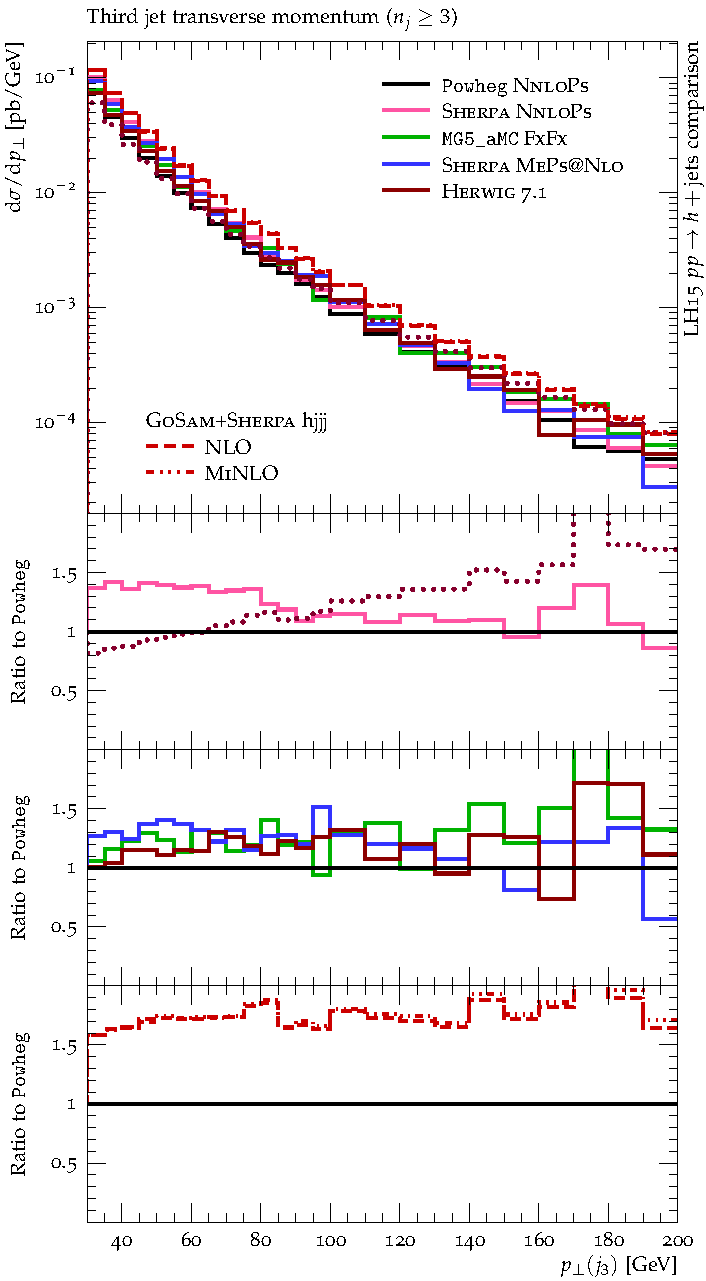
\includegraphics[width=0.47\textwidth]{figures/hjetscomp_u_jet3_pT_incl.pdf}
  \hfill
  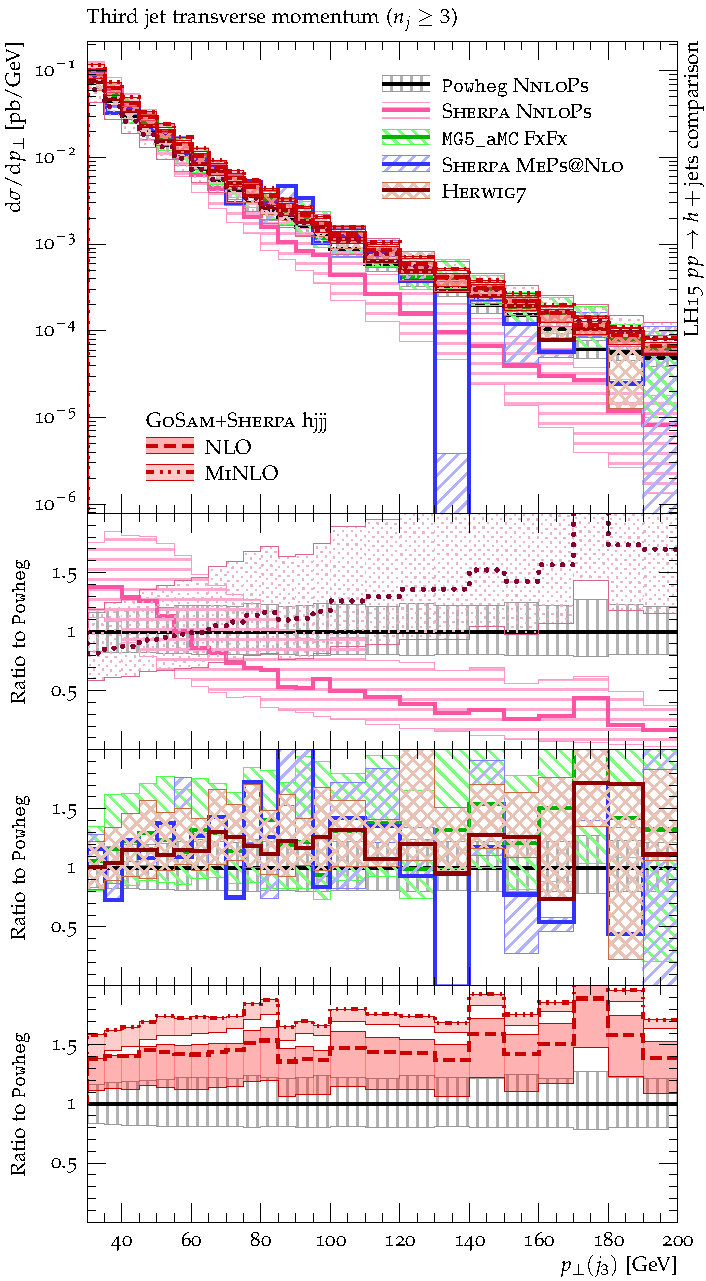
\includegraphics[width=0.47\textwidth]{figures/hjetscomp_jet3_pT_incl.pdf}
  \caption{
    The third jet transverse momentum distribution for $H+\ge3$ jets
    shown without (left) and with (right) theoretical uncertainty bands.
    \label{fig:hjetscomp:results:mobs:j3pt}
  }
\end{figure}

The third jet $p_T$ for $H+\ge3$ jets is shown in
Figure~\ref{fig:hjetscomp:results:mobs:j3pt}. MG5, Herwig7 and Sherpa
tend to be higher than Powheg (where the jet is produced by a parton
shower), but lower than that from Gosam $H+\ge3$ jets, which has the
correct NLO $K$-factor. The multijet phase space results in smaller
Sudakov effects, and thus better agreement with the fixed-order
predictions.

\begin{figure}[t!]
  \centering
  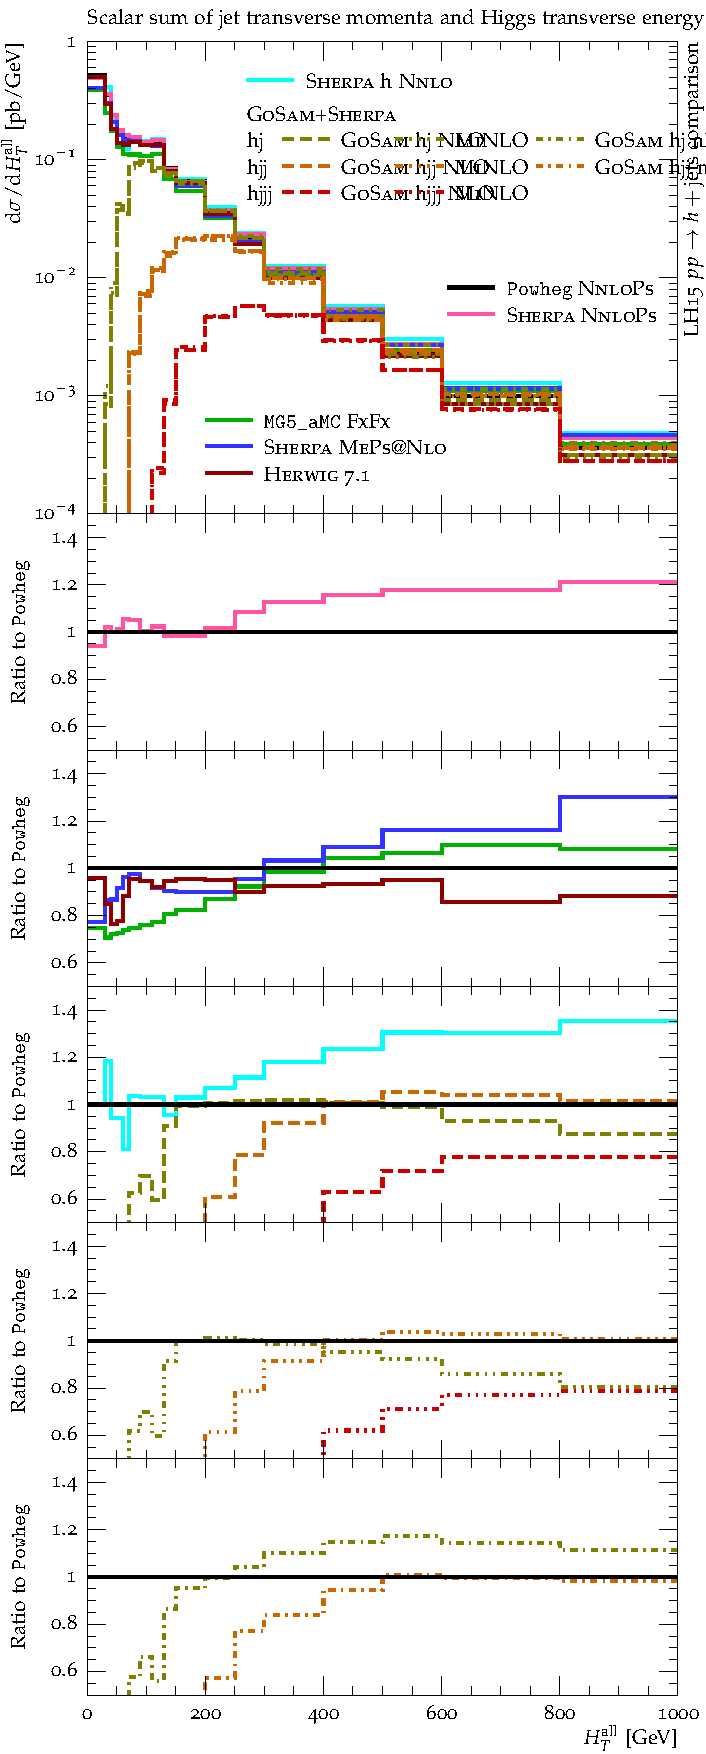
\includegraphics[width=0.47\textwidth]{figures/hjetscomp_u_HT_all.pdf}
  \hfill
  \includegraphics[width=0.47\textwidth]{figures/hjetscomp_HT_all.pdf}
  \caption{
    The $H_T$ distribution for $H+\ge1$ jets \Todo{is this correct?}
    without (left) and with (right) uncertainties.
    \label{fig:hjetscomp:results:mobs:HT_all}
  }
\end{figure}

\begin{figure}[t!]
  \centering
  \includegraphics[width=0.47\textwidth]{figures/hjetscomp_u_HT_jets.pdf}
  \hfill
  \includegraphics[width=0.47\textwidth]{figures/hjetscomp_HT_jets.pdf}
  \caption{
    The $H_{T,\mathrm{jets}}$ distribution for $H+\ge1$ jet final
    states, without (left) and with (right) uncertainties.
    \label{fig:hjetscomp:results:mobs:HT_jets}
  }
\end{figure}

The $H_T$ distribution (sum of the transverse momenta for all objects
in the final state) for $H+\ge1$ jets is shown in
Figure~\ref{fig:hjetscomp:results:mobs:HT_all} and the $H_T$
distribution for jets only is shown in in
Figure~\ref{fig:hjetscomp:results:mobs:HT_jets}. \Todo{Jan: we don't
  consider $H$ decays, so the all-objects HT would be different from
  an experimental point of view. Do we want both HTs and clarify or
  only the HTjets.}
MG5 and Sherpa tend to be lower than Powheg at low $H_T$ and higher at
large $H_T$. The fixed order predictions (from gosam and from $H+\ge1$
jet at NNLO) are consistently lower than Powheg (although the NNLO
prediction does agree with Powheg in the 150-300 GeV range for
$HT_{jets}$).



\clearpage
\subsection{Jet veto cross sections}
\label{sec:hjetscomp:results:jvobs}

This section is concerned with the cummulative jet veto cross sections. 
In the first three cases, Figures 
\ref{fig:hjetscomp:results:jvobs:jvxs0}-\ref{fig:hjetscomp:results:jvobs:jvxs1j200}, 
additional radiation is vetoed by means of a maximal transverse 
momentum of the (sub)leading jet, $p_\perp^\text{veto}$. These 
observables recover the respective inclusive cross section as 
$p_\perp^\text{veto}\to\infty$. In this region, the fixed order 
part of the respective calculations dominates the cross section 
and associated uncertainties. The opposite regime, $p_\perp^\text{veto}\to 0$, 
is a classic example of a resummation dominated observable. Here, the 
properties of the respective parton showers come fully into play and 
differences are largely due to their characteristics. The last case 
investigated is cross section after VBF cuts when vetoing additional 
central jet activity in dependence of the rapidity distance of the 
tagging jet pair, $y_\text{dist}<y_\text{dist}^\text{max}$. Here, 
DGLAP-type resummation regions are present throughout the spectrum and 
this observable should be ideal to study BFKL-like dynamics.

\begin{figure}[t!]
  \centering
  \includegraphics[width=0.47\textwidth]{figures/hjetscomp_u_xs_jet_veto_j0.pdf}
  \hfill
  \includegraphics[width=0.47\textwidth]{figures/hjetscomp_xs_jet_veto_j0.pdf}
  \caption{
    The exclusive zero jet cross section as a function of 
    the vetoed minimal leading jet transverse momentum,
    without (left) and with (right) uncertainties.
    \label{fig:hjetscomp:results:jvobs:jvxs0}
  }
\end{figure}

We start by considering 
the cross section for the production of a Higgs boson and no 
additional jets as a function of the minimum jet transverse momentum 
is shown in Figure~\ref{fig:hjetscomp:results:jvobs:jvxs0}. Remarkable 
agreement between both \NNLOPS simulations and the dedicated resummation 
of STWZ is found, typically well with 5\% within the considered range. 
However, as both \NNLOPS' resummation accuracy is limited by their parton 
shower's accuracy and both do not (\Powheg) or only partially (\Sherpa) 
assess their intrinsic uncertainty and interplay with the hard process' 
scale variations, their uncertainties remain much larger than those of 
STWZ. The multijet merged calculations show a wider spread. In addition to 
suffering from their NLO normalisation in the $p_\perp^\text{veto}\to\infty$ 
limit, they show different behaviour as $p_\perp^\text{veto}\to 0$. Here, 
\Sherpa \MEPSatNLO exhibits more QCD activity than the other computations. 

\begin{figure}[t!]
  \centering
  \includegraphics[width=0.47\textwidth]{figures/hjetscomp_u_xs_jet_veto_j1_30.pdf}
  \hfill
  \includegraphics[width=0.47\textwidth]{figures/hjetscomp_xs_jet_veto_j1_30.pdf}
  \caption{
    The cross section for events containing a Higgs boson 
    and one jet with $p_\perp>30\,\gev$ as a function of
    the vetoed minimal second jet transverse momentum without
    (left) and with (right) uncertainties.
    \label{fig:hjetscomp:results:jvobs:jvxs1j30}
  }
\end{figure}

\begin{figure}[t!]
  \centering
  \includegraphics[width=0.47\textwidth]{figures/hjetscomp_u_xs_jet_veto_j1_200.pdf}
  \hfill
  \includegraphics[width=0.47\textwidth]{figures/hjetscomp_xs_jet_veto_j1_200.pdf}
  \caption{
    The cross section for events containing a Higgs boson 
    and one jet with $p_\perp>200\,\gev$ as a function of
    the vetoed minimal second jet transverse momentum without
    (left) and with (right) uncertainties.
    \label{fig:hjetscomp:results:jvobs:jvxs1j200}
  }
\end{figure}

Next, we require the presence of at least one jet with 
a minimal transverse momentum of $30$ and $200$ \gev, respectively. 
The cross section as a function of 
the sub-leading jets maximal transverse momentum is displayed in 
Figure~\ref{fig:hjetscomp:results:jvobs:jvxs1j30} and 
Figure~\ref{fig:hjetscomp:results:jvobs:jvxs1j200}, respectively. 
Before starting the discussion it worthy to note that although all parton 
shower matched or merged calculations have the same accuracy as 
$p_\perp^\text{veto}\to\infty$ and in the resummation dominated region, 
the multijet merged calculation possess a better description of the 
second jet emission and thus should lead to more accurate results 
throughout the spectrum provided the merging systematics are under control. 
Currently employed uncertainty estimates, however, will not reflect this 
as resummation uncertainties are not assessed or only incompletely assessed.

Putting no special requirements on the leading jet, cf.\ Figure 
\ref{fig:hjetscomp:results:jvobs:jvxs1j30}, good agreement 
between all calculations is found. The \NNLOPS ones agreen again within 
5\% of one another with very similar uncertainties. This is noteworthy 
in sofar as, in comparison with the results of 
Figure~\ref{fig:hjetscomp:results:jvobs:jvxs0}, both calculations' 
accuracies have degraded by one order. The multijet merged calculations 
also show a similar behaviour as in the previous case, also showing the 
same features as before: \MGaMC exhibits a smaller cross section due to 
its scale choice while \Sherpa \MEPSatNLO predicts more soft radiation. 
Only the slight relative lack of small $p_\perp$ radiation is more 
pronounced in \Herwig now. Again, the uncertainties of \MGaMC and \Sherpa 
are of similar size while \Herwig's are somewhat smaller than the \NNLOPS 
ones, especially in the resummation dominated region as 
$p_\perp^\text{veto}\to 0$.

Raising the requirements on the leading jet to $200$ \gev in Figure 
\ref{fig:hjetscomp:results:jvobs:jvxs1j200} now shows clear distinctions 
between the different calculations now. Among the \NNLOPS calculations, 
\Sherpa starts out at a higher asymtotic cross section but remains within 
20\% and of \Powheg, the respective uncertainties covering one another. 
The multijet merged calculations show \Herwig largely agreeing with 
\Powheg with a constant offset of $-10\%$ and the familiar lower 
probability of low-$p_\perp$ jet emissions. \Sherpa \MEPSatNLO's 
asymtotic cross section is as large as the \Sherpa \NNLOPS one and, 
unsurprisingly due to the use of the same parton shower, shows a 
similar radiation pattern for a large range. As before, it exhibits 
a relative overabundance of soft jet radiation. Lastly, \MGaMC's 
asymtotic cross section now is the same level as \Powheg's, despite 
its higher scale choice. The pattern of the uncertainties, however, 
remains the same as before.

\Todo{The central jet veto cross sections are a mess. Looking into the 
      analysis this is Ivan's code. It defines $y_\text{dist}$ as the 
      minimal rapidity distance between the centre of the forward and 
      backward jets and any jet inbetween,
      $$
	y_\text{dist}\;=\;\min\limits_{j|y(j_\text{bw})<y(j)<y(j_\text{fw})}
	                  \left|y(j)-\frac{y_\text{fw}+y_\text{bw}}{2}\right|\;.
      $$
      It can thus take the maximum value of $4.4$. The cummulative cross 
      section is then defined as 
      $\sigma_2(y_\text{dist}>y_\text{dist}^\text{min})$. Thus, this 
      observable vetoes events with too central additional radiation. 
      It has one flaw in the implementation, however, in the absence of 
      any third jet $y_\text{dist}$ is set to $>4.4$. Its asymtotic behaviour 
      at large $y_\text{dist}$ converges thus to the exclusive VBF 
      cross section, instead of zero. I just do not see what kind of 
      dynamics we are probing or what kind of relevance a construction 
      like this has. Especially since the forward backward jet are 
      generally not the VBF tagging jets. We do also have the same observable 
      in the pure dijet selection, which would then at least be nicely defined. 
      Only the effects there are even smaller. 
      Too many cooks, I guess. One should have had a recipe first.
      }


% \begin{figure}[t!]
%   \centering
%   \includegraphics[width=0.47\textwidth]{figures/hjetscomp_u_xs_central_jet_veto_VBF.pdf}
%   \hfill
%   \includegraphics[width=0.47\textwidth]{figures/hjetscomp_xs_central_jet_veto_VBF.pdf}
%   \caption{
%     The cross section after VBF cuts as a function of the maximal minimum 
%     rapidity distance of a central jet to the centre of the most forward 
%     and most backward jet.
%     \label{fig:hjetscomp:results:jvobs:cjvxsvbf}
%   }
% \end{figure}
% 
% \begin{figure}[t!]
%   \centering
%   \includegraphics[width=0.47\textwidth]{figures/hjetscomp_u_xs_central_jet_veto_VBF2.pdf}
%   \hfill
%   \includegraphics[width=0.47\textwidth]{figures/hjetscomp_xs_central_jet_veto_VBF2.pdf}
%   \caption{
%     The cross section after generalised VBF cuts as a function of the maximal minimum 
%     rapidity distance of a central jet to the centre of the most forward 
%     and most backward jet.
%     \label{fig:hjetscomp:results:jvobs:cjvxsvbf2}
%   }
% \end{figure}
% 
% Finally, we consider the cross section after VBF cuts applying a veto 
% on additional central jet activity with $p_\perp>30\,\gev$ in dependence 
% of the maximal rapidity distance of the tagging jets, 
% $y_\text{dist}<y_\text{dist}^\text{max}$, as displayed in 
% Figure \ref{fig:hjetscomp:results:jvobs:cjvxsvbf}. Here, all parton shower based 
% resummation calculations give very similar results with \MGaMC possessing 
% a reduced cross section due to its scale choice. \Hej, being based on 
% BFKL dynamics, does not deviate substantially in its predicted shape. 
% However, its cross section is reduced by a constant 50-60\%. Alternatively, 
% when applying the generalised version of the VBF cuts, labelled VBF2, 
% a similar picture presents itself in 
% Figure \ref{fig:hjetscomp:results:jvobs:cjvxsvbf2}. While, of course, the 
% asymtotic cross section at large $y_\text{dist}^\text{max}$ coincides with 
% the one of the standard VBF cuts, for small $y_\text{dist}^\text{max}$ the 
% generalised VBF cuts allow for a much larger cross section.



